\documentclass{article}
\usepackage[margin=1in]{geometry}
\usepackage{amsmath, amssymb, amsthm}
\usepackage{hyperref}
\usepackage{nicefrac}
\usepackage{xcolor}
\usepackage[sort]{natbib}
\usepackage{pgfplots}

\setlength{\parskip}{2mm}

\newtheorem{theorem}{Theorem}[subsection]
\newtheorem{corollary}{Corollary}[subsection]
\newtheorem{lemma}{Lemma}[subsection]

\theoremstyle{remark}
\newtheorem*{remark}{Remark}

\newcommand{\comprule}{\textcolor[RGB]{220,220,220}{\rule{\linewidth}{0.2pt}}}

\newcommand{\real}{\mathbb{R}}
\newcommand{\Exp}{\mathbb{E}}
\newcommand{\Var}{\mathrm{Var}}
\newcommand{\Cov}{\mathrm{Cov}}
\newcommand{\inner}[2]{\left\langle #1, #2 \right\rangle}
\newcommand{\indic}[1]{\mathbf{1}_{\{#1\}}}

\newcommand{\calN}{\mathcal{N}}
\newcommand{\calE}{\mathcal{E}}

\newcommand{\vscomment}[1]{\textcolor{blue}{#1}}
\newcommand{\TODO}{\textcolor{red}{TODO}}

\title{Notes for High-Dimensional Probability\footnote{\citet{vershynin2019high}}}
\author{Vishwak Srinivasan}

\date{}

\begin{document}
\raggedright

\maketitle
\tableofcontents

\newpage

\section{Preliminaries}
\subsection{Example on approximate Caratheodory's Theorem}

First, we begin by discussing Caratheodory's Theorem:
\begin{theorem}[Caratheodory's Theorem]
\label{thm:approx-caratheodory}
Consider a convex set \(S \subseteq \real^{p}\). Any point \(x \in S\) can be represented as a convex combination of at most \(p + 1\) distinct points from \(S\).
\end{theorem}

\begin{remark}
This result is a popular result in convex analysis, and is tight. The tight lower bound is achieved by a simplex in \(p\) dimensions, which corresponds to \(p + 1\) vertices.
\end{remark}

Now, we seek an approximation of the above theorem like so: given \(k\) points \(\{x_{i}\}_{i=1}^{k} \subset S\), is it possible to approximate a point \(x \in S\)? We answer this in the affirmative below:
\begin{theorem}[Approx. Caratheodory's Theorem]
Given \(x \in S \subseteq \real^{p}\), where \(S\) is convex, there exists a set of \(k\) points \(\{x_{i}\}_{i=1}^{k} \in S\), such that the following holds:
\begin{equation*}
\left\|x - \frac{1}{k}\sum_{i=1}^{k}x_{i}\right\|_{2} \leq \frac{\mathrm{diam}(S)}{\sqrt{k}}
\end{equation*}
where \(\mathrm{diam}(S) = \sup\limits_{s, t \in S} \|s - t\|_{2}\).
\end{theorem}

\begin{proof}
By the fact that \(x \in S\), we know that we can write \(x\) as a convex combination of a subset \(\{z_{i}\}_{i=1}^{m}\) that satisfy \(\mathrm{CONV}(\{z_{i}\}_{i=1}^{m}) = S\), where \(m \leq p + 1\). Let the coefficients be \(\{\lambda_{i}\}_{i=1}^{m}\) where \(\sum\limits_{i=1}^{m} \lambda_{i} = 1\) and \(\lambda_{i} \geq 0\) for all \(i \in [m]\).

Consider a random variable \(Z\) that takes \(m\) different values from the set \(\{z_{i}\}_{i=1}^{m}\) with probability \(\lambda_{i}\). Note that \(\Exp[Z] = x\), since \(\Exp[Z] = \sum\limits_{i=1}^{m} \Pr(Z = z_{i})z_{i} = \sum\limits_{i=1}^{m} \lambda_{i}z_{i} = x\).

We know that for any \(x \in \real^{p}\) and independent random variables \(\{Z_{i}\}_{i=1}^{k}\) that satisfy \(\Exp[Z_{i}] = x\) for all \(i \in [k]\):
\begin{align*}
\Exp\left[\left\|x - \frac{1}{k}\sum_{i=1}^{k}Z_{i}\right\|_{2}^{2}\right] &= \Exp\left[\left\|\frac{1}{k}\sum_{i=1}^{k}(x - Z_{i})\right\|_{2}^{2}\right] \\
&= \frac{1}{k^{2}}\Exp\left[\left\|\sum_{i=1}^{k} (x - Z_{i})\right\|_{2}^{2}\right] \\
&\overset{(i)}= \frac{1}{k^{2}}\sum_{i=1}^{k}\Exp\left[\left\|x - Z_{i}\right\|_{2}^{2}\right] \\
&\overset{(ii)}\leq \frac{1}{k^{2}}\sum_{i=1}^{k}\mathrm{diam}(S)^{2} = \frac{\mathrm{diam}(S)^{2}}{k}
\end{align*}
Step \((i)\) holds true due to Lemma \ref{lem:zero-mean-norm}. Step \((ii)\) follows from the fact that \(Z_{i}, x \in S\) which implies that \(\|Z_{i} - x\|_{2} \leq \mathrm{diam}(S)\) followed by the fact that \(\Exp[c] = c\) for constant \(c\).

Therefore, there exists a realization of \(\{Z_{i}\}_{i=1}^{k}\), that satisfies:
\begin{equation*}
\left\|x - \frac{1}{k}\sum_{i=1}^{k}Z_{i}\right\|_{2} \leq \frac{\mathrm{diam}(S)}{\sqrt{k}}
\end{equation*}
\end{proof}

\begin{remark}
First note the dimension independence in the result. Secondly, in the special case where \(S\) consists of elements with bounded norms i.e., \(\|x\|_{2} \leq B\) for all \(x \in S\), the diameter of the set is bounded by \(2B\) by an application of the triangle inequality. Finally, note that if we have \(k \to \infty\) samples from the set, then our approximation is going to be perfect.
\end{remark}

The method used to prove Theorem \ref{thm:approx-caratheodory} is called Maurey's Empirical Method.

\subsubsection{Auxiliary Lemmata}

\begin{lemma}
\label{lem:zero-mean-norm}
Let \(\{X_{i}\}_{i=1}^{k}\) be a set of independent zero-mean random variables. The following holds true:
\begin{equation*}
\Exp\left[\left\|\sum_{i=1}^{k}X_{i}\right\|_{2}^{2}\right] = \sum_{i=1}^{k}\Exp\left[\left\|X_{i}\right\|_{2}^{2}\right]
\end{equation*}
\end{lemma}

\begin{proof}
First note that:
\begin{align*}
\left\|\sum_{i=1}^{k}X_{i}\right\|_{2}^{2} &= \inner{\sum_{i=1}^{k}X_{i}}{\sum_{j=1}^{k}X_{j}} \\
&= \sum_{i=1}^{k}\sum_{j=1}^{k}X_{i}^{T}X_{j} \\
&= \sum_{i=1}^{k}\|X_{i}\|_{2}^{2} + 2\sum_{\substack{i, j = 1 \\ i \neq j}}^{k}X_{i}^{T}X_{j}
\end{align*}

Taking expectations on both sides:
\begin{align*}
\Exp\left[\left\|\sum_{i=1}^{k}X_{i}\right\|_{2}^{2}\right] &= \Exp\left[\sum_{i=1}^{k}\|X_{i}\|_{2}^{2}\right] + 2\Exp\left[\sum_{\substack{i, j = 1 \\ i \neq j}}^{k}X_{i}^{T}X_{j}\right] \\
&= \sum_{i=1}^{k}\Exp\left[\left\|X_{i}\right\|_{2}^{2}\right] + 2\sum_{\substack{i, j = 1 \\ i \neq j}}^{k} \Exp\left[X_{i}^{T}X_{j}\right]
\end{align*}

Since \(X_{i}\)s are independent, \(\Exp\left[X_{i}^{T}X_{j}\right] = \Exp\left[X_{i}\right]^{T}\Exp\left[X_{j}\right] = 0\), and this completes the proof.
\end{proof}

\begin{lemma}
For all integers \(m \in [1, n]\), we have the following series of inequalities:
\begin{equation*}
\left(\frac{n}{m}\right)^{m} \leq \binom{n}{m} \leq \sum_{k=0}^{m}\binom{n}{m} \leq \left(\frac{en}{m}\right)^{m}
\end{equation*}
\end{lemma}

\begin{proof}
First inequality:
\begin{equation*}
\binom{n}{m} m^{m} = \frac{n!}{(n - m)! \cdot m!} m^{m} \geq \frac{n!}{(n - m)!} \geq n^{m} \Rightarrow \binom{n}{m} \geq \left(\frac{n}{m}\right)^{m}
\end{equation*}

Second inequality:
\begin{equation*}
\binom{n}{m} \leq \binom{n}{m} + \sum_{k=0}^{m-1} \binom{n}{k} = \sum_{k=0}^{m}\binom{n}{k}
\end{equation*}

Third inequality:
\begin{equation*}
\left(\frac{m}{n}\right)^{m} \sum_{k=0}^{m}\binom{n}{k} \leq \sum_{k=0}^{m} \binom{n}{k} \left(\frac{m}{n}\right)^{k} \leq \sum_{k=0}^{n} \binom{n}{k} \left(\frac{m}{n}\right)^{k} = \left(1 + \frac{m}{n}\right)^{n} \leq e^{m} \Rightarrow \sum_{k=0}^{m}\binom{n}{k} \leq \left(\frac{en}{m}\right)^{m}
\end{equation*}
\end{proof}

\subsection{Quantities and Inequalities associated with RVs}

\begin{itemize}
\item Expectation: \(\Exp[X]\)
\item Variance: \(\Var[X] = \Exp[(X - \Exp[X])^{2}]\)
\item MGF: \(M_{X}(t) = \Exp[e^{tX}]\), \(t \in \real\)
\item \(p^{th}\) moment: \(\Exp[X^{p}]\) and \(p^{th}\) absolute moment: \(\Exp[|X|^{p}]\)
\item \(L^{p}\) norm: \(\|X\|_{L^{p}} = \sqrt[p]{\Exp[|X|^{p}]}\)
\item \(L^{\infty}\) norm: \(\|X\|_{L^{\infty}} = \mathrm{ess} \sup |X|\), where \(\mathrm{ess} \sup |X|\) denotes the supremum over all set with measure not 0. Also note that: \(\mathrm{ess} \sup |X| \leq \sup |X|\).
\item Covariance: \(\Cov(X, Y) = \Exp[(X - \Exp[X])(Y - \Exp[Y])]\)
\item CDF: \(F_{X}(t) = \Pr(X \leq t)\), \(t \in \real\)
\end{itemize}

For a convex function \(f\) and any random variable \(X\), we have by \emph{Jensen's inequality} that:
\begin{equation*}
f(\Exp[X]) \leq \Exp[f(X)]
\end{equation*}

Consequently, for a concave function \(f\) and any random variable \(X\), we have:
\begin{equation*}
f(\Exp[X]) \geq \Exp[f(X)]
\end{equation*}

As a special case, consider \(f(x) : x^{\nicefrac{q}{p}}\) where \(q > p\). Note that \(f\) is convex. Therefore:
\begin{equation*}
(\Exp\left[|X|^{p}\right])^{\nicefrac{q}{p}} \leq \Exp\left[|X|^{q}\right] \Rightarrow \|X\|_{L^{p}} \leq \|X\|_{L^{q}}
\end{equation*}

Another inequality is the \emph{Cauchy-Schwarz inequality}, which states that for any two RVs \(X\) and \(Y\):
\begin{equation*}
\Exp[|XY|] \leq \sqrt{\Exp[X^{2}]}\sqrt{\Exp[Y^{2}]} = ||X||_{L^{2}} ||Y||_{L^{2}}
\end{equation*}

We also have \emph{Holder's inequality} which generalizes \emph{Cauchy-Schwarz} to dual norms as:
\begin{equation*}
\Exp[|XY|] \leq ||X||_{L^{p}} ||Y||_{L^{q}} \qquad;\qquad \frac{1}{p} + \frac{1}{q} = 1
\end{equation*}

The following lemma characterizes the expectation as a quantity involving only tails:
\begin{lemma}
\label{lem:tail-expectation}
Consider a non-negative random variable \(X\). The expectation of this random variable can be written as:
\begin{equation*}
\Exp[X] = \int_{0}^{\infty} \Pr(X > t) dt
\end{equation*}
\end{lemma}

\begin{proof}
For any \(x \geq 0\), we have that:
\begin{equation*}
x = \int_{0}^{\infty} \indic{t < x} dt = \int_{0}^{x} 1 dt + \int_{x}^{\infty} 0 dt
\end{equation*}

Therefore:
\begin{align*}
X = \int_{0}^{\infty} \indic{t < X} dt \Rightarrow \Exp[X] &= \Exp\left[\int_{0}^{\infty} \indic{t < X} dt\right] \\
& = \int_{0}^{\infty} \int_{-\infty}^{\infty} \indic{t < x} \Pr(X = x) dx dt \\
& = \int_{0}^{\infty} \int_{t}^{\infty} \Pr(X = x) dx dt \\
& = \int_{0}^{\infty} \Pr(X > t) dt
\end{align*}
\end{proof}

A simple generalization for real-valued random variables from the proof of Lemma \ref{lem:tail-expectation} is as follows:
\begin{corollary}
Consider a real valued random variable \(X\). The expectation of this random variable can be written as:
\begin{equation*}
\Exp[X] = \int_{0}^{\infty} \Pr(X > t) dt - \int_{-\infty}^{0} \Pr(X < t) dt
\end{equation*}
\end{corollary}

An application of Lemma \ref{lem:tail-expectation} is to use it to bound the \(p^{th}\) absolute moments via tails:
\begin{corollary}
\label{cor:p-abs-moment}
For any random variable \(X\):
\begin{equation*}
\Exp\left[|X|^{p}\right] = \int_{0}^{\infty} pt^{p-1} \Pr(|X| > t) dt
\end{equation*}
\end{corollary}

Classical inequalities: Markov and Chebyshev's:
\begin{lemma}[Markov's Inequality]
Consider a non-negative random variable \(X\). Then the tails of \(X\) can be bounded as:
\begin{equation*}
\Pr(X > t) \leq \frac{\Exp[X]}{t}
\end{equation*}
\end{lemma}

\begin{proof}
Note that:
\begin{equation*}
\Exp[X] = \Exp[X \cdot \indic{X > t}] + \Exp[X \cdot \indic{X \leq t}] \geq \Exp[X \cdot \indic{X > t}] \geq t \Exp[\indic{X > t}] = t \Pr(X > t) \Rightarrow \Pr(X > t) \leq \frac{\Exp[X]}{t}
\end{equation*}
\end{proof}

\begin{corollary}[Chebyshev's Inequality]
Consider a random variable \(X\). Then the probability of deviation from the expectation of \(X\) can be bounded as:
\begin{equation*}
\Pr(|X - \Exp[X]| > t) \leq \frac{\Var(X)}{t^{2}}
\end{equation*}
\end{corollary}

\begin{proof}
Take \(Y = |X - \Exp[X]|\) as the random variable as apply Markov's inequality:
\begin{equation*}
\Pr(Y > t) = \Pr(Y^{2} > t^{2}) \leq \frac{\Exp[(X - \Exp[X])^{2}]}{t^{2}}
\end{equation*}
\end{proof}

\begin{remark}
Note that one can achieve better dependence on \(t\) by using higher moments - provided they exist:
\begin{equation*}
\Pr(Y > t) = \Pr(Y^{2k} > t^{2k}) \leq \frac{\Exp[(X - \Exp[X])^{2k}]}{t^{2k}}
\end{equation*}
\end{remark}

\subsection{Basic Limit Theorems}
\begin{theorem}[Strong Law of Large Numbers]
Let \(\{X_{i}\}_{i=1}^{n}\) be a sequence of identically and independently distributed random variables with mean \(\mu\). The quantity \(\bar{X}_{n} = \frac{1}{n}\sum\limits_{i=1}^{n} X_{i}\) satisfies:
\begin{equation*}
\bar{X}_{n} \xrightarrow{a.s.} \mu
\end{equation*}
as \(n \to \infty\).
\end{theorem}

Here \(\xrightarrow{a.s.}\) denotes \emph{almost sure convergence}, which is:
\begin{equation*}
\Pr\left(\lim_{n \to \infty} \bar{X}_{n} = \mu\right) = 1
\end{equation*}

There is a \emph{weak law of large numbers}, which can be derived from Chebyshev's Inequality, for distributions with bounded variance. It is stated below:
\begin{corollary}[Weak Law of Large Numbers]
Let \(\{X_{i}\}_{i=1}^{n}\) be a sequence of identically and independently distributed random variables with mean \(\mu\) and variance \(\sigma^{2} < \infty\). The quantity \(\bar{X}_{n} = \frac{1}{n}\sum\limits_{i=1}^{n} X_{i}\) satisfies:
\begin{equation*}
\bar{X}_{n} \xrightarrow{p} \mu
\end{equation*}
where \(\xrightarrow{p}\) denotes \emph{convergence in probability}, which is;
\begin{equation*}
\forall \epsilon > 0, \qquad \lim_{n \to \infty} \Pr\left(|\bar{X}_{n} - \mu| > \epsilon\right) = 0
\end{equation*}
\end{corollary}

\begin{proof}
First note \(\Exp\left[\bar{X}_{n}\right] = \mu\), and hence \(\Var(\bar{X}_{n}) = \frac{1}{n^{2}}\Var\left(\sum\limits_{i=1}^{n}X_{i}\right) = \frac{1}{n^{2}}\sum\limits_{i=1}^{n}\Var\left(X_{i}\right) = \frac{\sigma^{2}}{n}\).

By Chebyshev's inequality, for any \(\epsilon > 0\):
\begin{equation*}
\Pr(|\bar{X}_{n} - \mu| > \epsilon) \leq \frac{\sigma^{2}}{n\epsilon} \Rightarrow \lim_{n \to \infty} \Pr(|\bar{X}_{n} - \mu| > \epsilon) = 0 \enskip (\because \text{Sandwich theorem})
\end{equation*}
\end{proof}

\begin{remark}
This weak result is \emph{weak} because \(\xrightarrow{a.s.}\) implies \(\xrightarrow{p.}\).
\end{remark}

\comprule

Next, we state a result that gives the asymptotic distribution of \(\bar{X}_{n}\).
\begin{theorem}[Central Limit Theorem]
\label{thm:clt}
Let \(\{X_{i}\}_{i=1}^{n}\) be a sequence of identically and independently distributed random variables with mean \(\mu\) and variance \(\sigma^{2} < \infty\). Define \(\bar{X}_{n} = \frac{1}{n}\sum\limits_{i=1}^{n} X_{i}\). Then:
\begin{equation*}
\frac{\sqrt{n}(\bar{X}_{n} - \mu)}{\sigma} \xrightarrow{d} \calN(0, 1) \qquad \text{as } n \to \infty
\end{equation*}
\end{theorem}

While this result states that the deviation between the sample mean and population mean is 0 in the limit, we can give some non asymptotic guarantees on the deviation as follows:
\begin{lemma}
Let \(\{X_{i}\}_{i=1}^{n}\) be a sequence of identically and independently distributed random variables with mean \(\mu\) and variance \(\sigma^{2} < \infty\). We have that:
\begin{equation*}
\Exp\left[\left|\frac{1}{n}\sum_{i=1}^{n}X_{i} - \mu\right|\right] = O\left(\frac{1}{\sqrt{n}}\right)
\end{equation*}
\end{lemma}

\begin{proof}
By Jensen's inequality:
\begin{equation*}
\Exp\left[|Z|\right] \leq \sqrt{\Exp\left[Z^{2}\right]}
\end{equation*}
(Note that this also follows from the fact that \(\|Z\|_{L^{1}} \leq \|Z\|_{L^{2}}\))

Therefore:
\begin{align*}
\Exp\left[\left|\frac{1}{n}\sum_{i=1}^{n}X_{i} - \mu\right|\right] &\leq \sqrt{\Exp\left[\left(\frac{1}{n}\sum_{i=1}^{n}X_{i} - \mu\right)^{2}\right]} \\
&= \sqrt{\Exp\left[\left(\frac{1}{n}\sum_{i=1}^{n}(X_{i} - \mu)\right)^{2}\right]} \\
&= \sqrt{\frac{1}{n^{2}}\Exp\left[\left(\sum_{i=1}^{n}(X_{i} - \mu)\right)^{2}\right]} \\
&\overset{(i)}= \sqrt{\frac{1}{n^{2}}\sum_{i=1}^{n}\Exp\left[(X_{i} - \mu)^{2}\right]} \\
&= \sqrt{\frac{\sigma^{2}}{n}} = O\left(\frac{1}{\sqrt{n}}\right)
\end{align*}
where Step \((i)\) follows from Lemma \ref{lem:zero-mean-norm} for 1-D random variables.
\end{proof}

A special case of the Central Limit Theorem is to provide approximate distributions for binomial distributions. Recall that the binomial distribution \(\mathrm{Bin}(n, p)\) is the sum of \(n\) independent Bernoulli distribution with parameter \(p\). Therefore, we get that:
\begin{equation*}
\frac{\sqrt{n}(\bar{X}_{n} - \mu)}{\sigma} = \frac{n\bar{X}_{n} - n\mu}{\sigma\sqrt{n}} = \frac{B_{n, p} - np}{\sqrt{n}\sqrt{p(1 - p)}} \xrightarrow{d} \calN(0, 1) \enskip \text{as } n \to \infty
\end{equation*}
where \(X_{i} \sim \mathrm{Ber}(p), i \in [n]\) and \(B_{n, p} \sim \mathrm{Bin}(n, p)\). This means that \(B_{n, p} \xrightarrow{d} \calN(np, np(1 - p))\) as \(n \to \infty\).

However, there is a better limit theorem in the regime where \(p \to \infty, n \to \infty\) and \(np = \lambda > 0\). This is the Poisson Limit Theorem:
\begin{theorem}[Poisson Limit Theorem]
\label{thm:plt}
Consider \(\{X_{i}\}_{i=1}^{n}\) to be \(n\) independent Bernoulli variables with parameters \(p_{i}\). Then, for \(n \to \infty\), \(\max\limits_{i \in [n]} p_{i} \to 0\) and \(\sum\limits_{i=1}^{n}p_{i} = \lambda > 0\), we have that:
\begin{equation*}
\sum_{i=1}^{n}X_{i} \xrightarrow{d} \mathrm{Poi}(\lambda)
\end{equation*}
\end{theorem}

\begin{remark}
In the special case when all \(p_{i}\)s are equal, we obtain the same result with \(n \to \infty\), \(p \to 0\) and \(np = \lambda > 0\) as described informally earlier.
\end{remark}

\newpage

\section{Concentration inequalities}
\subsection{Basic Gaussian Inequalities}
\begin{lemma}[Mill's inequalities]
Let \(g \sim \calN(0, 1)\). We have the following lower and upper bounds for the tail \(\Pr(g > t)\), \(t > 0\) as follows:
\begin{equation*}
\left(\frac{1}{t} - \frac{1}{t^{3}}\right)\frac{1}{\sqrt{2\pi}}e^{-\nicefrac{t^{2}}{2}} \leq \Pr(g > t) \leq \frac{1}{t}\cdot\frac{1}{\sqrt{2\pi}}e^{-\nicefrac{t^{2}}{2}}
\end{equation*}
\end{lemma}

\begin{proof}
First, the upper bound:
\begin{align*}
\Pr(g > t) &= \frac{1}{\sqrt{2\pi}}\int_{t}^{\infty} e^{-\nicefrac{x^{2}}{2}} dx \\
&= \frac{1}{t} \cdot \frac{1}{\sqrt{2\pi}}\int_{t}^{\infty} te^{-\nicefrac{x^{2}}{2}} dx \\
&\leq \frac{1}{t} \cdot \frac{1}{\sqrt{2\pi}}\int_{t}^{\infty} xe^{-\nicefrac{x^{2}}{2}} dx \\
&= \frac{1}{t} \cdot \frac{1}{\sqrt{2\pi}}\int_{\nicefrac{t^{2}}{2}}^{\infty} ye^{-y} dy \qquad \left(\because y = \frac{x^{2}}{2}\right)\\
&= \frac{1}{t} \cdot \frac{1}{\sqrt{2\pi}}e^{-\nicefrac{t^{2}}{2}}
\end{align*}

Second, the lower bound:
\begin{align*}
\Pr(g > t) &= \frac{1}{\sqrt{2\pi}}\int_{t}^{\infty} e^{-\nicefrac{x^{2}}{2}} dx \\
&\geq \frac{1}{\sqrt{2\pi}}\int_{t}^{\infty} \left(1 - \frac{3}{x^{4}}\right)e^{-\nicefrac{x^{2}}{2}} dx \qquad \left(\because 1 - \frac{3}{x^{4}} \leq 1 \enskip \forall \enskip x > 0\right) \\
&\geq \left(\frac{1}{t} - \frac{1}{t^{3}}\right)\frac{1}{\sqrt{2\pi}}e^{-\nicefrac{t^{2}}{2}}
\end{align*}

An alternative proof for the lower bound can be obtained as follows. First note that for \(\phi(z) = \frac{1}{\sqrt{2\pi}}e^{-\nicefrac{z^{2}}{2}}\), we have (see \citep{wainwright2019high}):
\begin{equation*}
\phi'(z) = \frac{1}{\sqrt{2\pi}} \cdot -ze^{\nicefrac{-z^{2}}{2}} = -z\phi(z)
\end{equation*}

Therefore:
\begin{align*}
\Pr(g > t) &= \int_{t}^{\infty} \phi(x) dx \\
&= \int_{t}^{\infty} -\frac{\phi'(x)}{x} dx \\
&= \left. -\frac{1}{x}\phi(x)\right|_{t}^{\infty} - \int_{t}^{\infty} \frac{1}{x^{2}}\phi(x) dx \qquad \left(\because \text{int. by parts with } f(x) = -\frac{1}{x}, g(x) = \phi'(x)\right)\\
&= \frac{\phi(t)}{t} + \int_{t}^{\infty} \frac{1}{x^{3}}\phi'(x) dx \\
&= \frac{\phi(t)}{t} + \left.\frac{\phi(x)}{x^{3}}\right|_{t}^{\infty} + \underbrace{\int_{t}^{\infty} \frac{3}{x^{4}}\phi(x) dx}_{\geq 0} \qquad \left(\because \text{int. by parts with } f(x) = -\frac{1}{x^{3}}, g(x) = \phi'(x)\right)\\
&\geq \frac{\phi(t)}{t} - \frac{\phi(t)}{t^{3}}
\end{align*}
\end{proof}

\begin{remark}
Note that one can get tail bounds for \(\calN(0, \sigma^{2})\) by simply reparameterising the integrals as:
\begin{equation*}
\left(\frac{\sigma}{t} - \frac{\sigma}{t^{3}}\right)\frac{1}{\sqrt{2\pi}}e^{-\nicefrac{t^{2}}{2}} \leq \Pr(g > t) \leq \frac{\sigma}{t}\cdot\frac{1}{\sqrt{2\pi}}e^{-\nicefrac{t^{2}}{2}}
\end{equation*}
\end{remark}

\comprule

The Central Limit Theorem (Theorem \ref{thm:clt}) states that averages tend in distribution to a Gaussian. But what can be said about the distribution function itself? The following theorem gives this result:
\begin{theorem}[Berry-Esseen CLT]
Let \(\{X_{i}\}_{i=1}^{n}\) be a sequence of identically and independently distributed random variables with mean \(\mu\) and variance \(\sigma^{2} < \infty\). Define \(\bar{X}_{n} = \frac{1}{n}\sum\limits_{i=1}^{n} X_{i}\) and \(\bar{Z}_{n} = \sqrt{n}\frac{\bar{X}_{n} - \mu}{\sigma}\). Then:
\begin{equation*}
\left|\Pr(\bar{Z}_{n} > t) - \Pr(g > t))\right| \leq \frac{\rho}{\sqrt{n}}
\end{equation*}
where \(\rho = \frac{\Exp\left[|X_{i} - \mu|^{3}\right]}{\sigma^{3}}\), \(i \in [n]\) and \(g \sim \calN(0, 1)\).
\end{theorem}

\begin{remark}
This theorem basically states that the error of approximation scales as \(O\left(\frac{1}{\sqrt{n}}\right)\), which is bad, since we can't always leverage the normal approximation from the central limit theorem always.
\end{remark}

\subsubsection{Auxiliary Lemmata}
\begin{lemma}
Let \(g \sim \calN(0, 1)\). For \(t \geq 1\), we have that:
\begin{equation*}
\Exp\left[g^{2} \indic{g > t}\right] = \frac{t}{\sqrt{2\pi}}e^{-\nicefrac{t^{2}}{2}} + \Pr(g > t) \leq \left(t + \frac{1}{t}\right)\frac{1}{\sqrt{2\pi}}e^{-\nicefrac{t^{2}}{2}}
\end{equation*}
\end{lemma}

\begin{proof}
\begin{align*}
\Exp\left[g^{2} \indic{g > t}\right] &= \frac{1}{\sqrt{2\pi}}\int_{-\infty}^{\infty} x^{2} \indic{x > t} e^{-\nicefrac{x^{2}}{2}} dx \\
&= \frac{1}{\sqrt{2\pi}}\int_{t}^{\infty} x^{2} e^{-\nicefrac{x^{2}}{2}} dx \\
&= \frac{1}{\sqrt{2\pi}}\left(\left.\left(x \cdot e^{-x}\right)\right\rvert_{\nicefrac{t^{2}}{2}}^{\infty} + \int_{t}^{\infty} e^{-\nicefrac{x^{2}}{2}}dx\right) \qquad \left(\because \text{int. by parts with } f(x) = x, g(x) = xe^{-\nicefrac{x^{2}}{2}}\right) \\
&= \frac{t}{\sqrt{2\pi}}e^{-\nicefrac{t^{2}}{2}} + \Pr(g > t) \\
&\leq \frac{t}{\sqrt{2\pi}}e^{-\nicefrac{t^{2}}{2}} + \frac{1}{t}\cdot \frac{1}{\sqrt{2\pi}}e^{-\nicefrac{t^{2}}{2}} \\
&= \left(t + \frac{1}{t}\right)\frac{1}{\sqrt{2\pi}}e^{-\nicefrac{t^{2}}{2}}
\end{align*}
\end{proof}

\subsection{Hoeffding's Inequality}
First, we describe a simple bounded random variable namely the Rademacher random variable. \(X\) with support \(\{-1, +1\}\) is said to be distributed w.r.t. a Rademacher distribution if:
\begin{equation*}
\Pr(X = +1) = \Pr(X = -1) = \frac{1}{2}
\end{equation*}

Let's discuss about the basic quantities attributed to a random variable. Note that \(\Exp[X] = 0\) and \(\Var[X] = \frac{1}{2}\). Also the moment generating function is:
\begin{equation*}
M_{X}(t) = \Exp\left[e^{tX}\right] = \frac{1}{2}e^{t} + \frac{1}{2}e^{-t} = \cosh(t)
\end{equation*}

We have the first concentration inequality for these random variables.
\begin{theorem}
\label{thm:rademacher-hoeffding}
Let \(\{X_{i}\}_{i=1}^{n}\) be a sequence of \(n\) i.i.d. Rademacher random variables. Then, for any \(a \in \real^{n}\) we have:
\begin{equation*}
\Pr\left(\sum_{i=1}^{n}a_{i}X_{i} > t\right) \leq \exp\left(-\frac{t^{2}}{2||a||_{2}^{2}}\right)
\end{equation*}
\end{theorem}

\begin{proof}
Let's begin with Markov's inequality:
\begin{align*}
\Pr\left(\sum_{i=1}^{n} a_{i}X_{i} > t\right) &= \Pr\left(\exp\left(s \cdot \sum_{i=1}^{n} a_{i}X_{i}\right) > \exp(s \cdot t)\right) \qquad (s > 0)\\
&\overset{(i)}\leq \frac{\Exp\left[\exp\left(s \cdot \sum\limits_{i=1}^{n} a_{i}X_{i}\right)\right]}{\exp(st)} \\
&= \frac{1}{\exp(st)} \Exp\left[\prod_{i=1}^{n} \exp(s \cdot a_{i}X_{i})\right] \\
&\overset{(ii)}= \frac{1}{\exp(st)} \prod_{i=1}^{n}\Exp\left[\exp(s \cdot a_{i}X_{i})\right] \\
&\overset{(iii)}= \frac{1}{\exp(st)} \prod_{i=1}^{n}\cosh(s\cdot a_{i}) \\
&\overset{(iv)}\leq \frac{1}{\exp(st)} \prod_{i=1}^{n}\exp\left(\frac{s^{2}a_{i}^{2}}{2}\right) \\
&= \frac{1}{\exp(st)} \exp\left(\frac{s^{2}||a||_{2}^{2}}{2}\right)
\end{align*}

Step \((i)\) uses Markov's inequality over \(Y = \exp\left(s \cdot \sum\limits_{i=1}^{n} a_{i}X_{i}\right)\). Step \((ii)\) uses the fact that \(X_{i}\)s are independent, and Step \((iii)\) uses the MGF derived earlier. Step \((iv)\) can be attributed to Lemma \ref{lem:cosh-upper}.

Therefore, we have shown for any \(s > 0\) that:
\begin{equation*}
\Pr\left(\sum_{i=1}^{n} a_{i}X_{i} > t\right) \leq \exp\left(s^{2}\frac{||a||_{2}^{2}}{2} - st\right)
\end{equation*}

To obtain the tighest / smallest upper bound, we minimize the RHS. The minimizer of the quadratic: \(s^{2}\frac{||a||_{2}^{2}}{2} - st\) w.r.t \(s\) is \(\frac{t}{||a||_{2}^{2}}\), resulting in:
\begin{equation*}
\Pr\left(\sum_{i=1}^{n} a_{i}X_{i} > t\right) \leq \exp\left(-\frac{t^{2}}{2||a||_{2}^{2}}\right)
\end{equation*}
\end{proof}

\begin{remark}
Note that the first step generally holds for any invertible function \(f\). We used such a trick in proving Chebyshev's inequality. Also note that since \(\Exp[X_{i}] = 0\) for all \(i \in [n]\), we didn't have an explicit mean term.

Also, in the case where \(a_{i} = \frac{1}{n}\) i.e., we care about the concentration of the sample average to the mean, we get:
\begin{equation*}
\Pr\left(\bar{X}_{n} > t\right) \leq \exp\left(-\frac{nt^{2}}{2}\right)
\end{equation*}

Generally, high probability guarantees are given by setting the RHS to a confidence parameter \(\delta\), like so:
\begin{equation*}
\bar{X}_{n} \leq \sqrt{\frac{2}{n}\log\left(\frac{1}{\delta}\right)} \qquad \text{w. p. } \geq 1 - \delta
\end{equation*}

Fix the error to \(\epsilon\). Smaller the \(\delta\), the more confident the estimate, but requires more samples.
\end{remark}

\comprule

There is a two sided version to this inequality as well, and the stated below:
\begin{corollary}
Let \(\{X_{i}\}_{i=1}^{n}\) be a sequence of \(n\) i.i.d. Rademacher random variables. Then, for any \(a \in \real^{n}\) we have:
\begin{equation*}
\Pr\left(\left|\sum_{i=1}^{n}a_{i}X_{i}\right| > t\right) \leq 2\exp\left(-\frac{t^{2}}{2||a||_{2}^{2}}\right)
\end{equation*}
\end{corollary}

\begin{proof}
Simple probability states that if for two events \(A\) and \(B\) such that \(A \Rightarrow B\), then \(\Pr(A) \leq \Pr(B)\). Therefore:
\begin{gather*}
\left|\sum_{i=1}^{n}a_{i}X_{i}\right| > t \Rightarrow \sum_{i=1}^{n}a_{i}X_{i} > t \vee \sum_{i=1}^{n}a_{i}X_{i} < -t \\
\Rightarrow \Pr\left(\left|\sum_{i=1}^{n}a_{i}X_{i}\right| > t\right) \leq \Pr\left(\sum_{i=1}^{n}a_{i}X_{i} > t \vee \sum_{i=1}^{n}a_{i}X_{i} < -t\right) \leq \Pr\left(\sum_{i=1}^{n}a_{i}X_{i} > t\right) + \Pr\left(\sum_{i=1}^{n}a_{i}X_{i} < -t\right) \\
\Rightarrow \Pr\left(\left|\sum_{i=1}^{n}a_{i}X_{i}\right| > t\right) \leq 2\exp\left(-\frac{t^{2}}{2||a||_{2}^{2}}\right)
\end{gather*}
\end{proof}

An interesting application of this inequality is as follows: say that you have a set of objects of two kinds, equally probably occuring. If you want to provide high probability guarantees on the number of objects of one kind, then you could use it as follows. For each object, assign \(Z_{i} = 1\) if the object is of the kind you want and \(0\) otherwise. Now, \(S_{n} = \sum\limits_{i=1}^{n} Z_{i}\) is the number of objects of the kind you desire. However, \(Z_{i}\) is supported on \(\{0, 1\}\), which means you would have to reparameterize. Note that:
\begin{equation*}
\Pr(S_{n} > t) = \Pr(2S - n > 2t - n) = \Pr\left(\sum_{i=1}^{n}(2Z_{i} - 1) > 2t - n\right) \leq \exp\left(-\frac{(2t - n)^{2}}{2n}\right)
\end{equation*}

So, if you anticipated having at least \(\frac{3}{4}n\) objects of the kind you want, then this would happen with probability at most \(e^{-\nicefrac{n}{8}}\).

Now the derivation above has given an idea of how to obtain bounds for \emph{bounded random variables} - of which the Rademacher random variable is an example. Below, we have a generalized theorem:
\begin{theorem}
\label{thm:bounded-hoeffding}
Let \(\{X_{i}\}_{i=1}^{n}\) be a sequence of \(n\) independent bounded random variables i.e., every \(X_{i}\) satisfies \(X_{i} \in [l_{i}, u_{i}]\). Then, we have that:
\begin{equation*}
\Pr\left(\sum_{i=1}^{n}(X_{i} - \Exp[X_{i}]) > t\right) \leq \exp\left(-\frac{2t^{2}}{||u - l||_{2}^{2}}\right)
\end{equation*}
\end{theorem}

\begin{proof}

The standard series of steps used in the proof of Theorem \ref{thm:rademacher-hoeffding} yields:
\begin{align*}
\Pr\left(\sum_{i=1}^{n}(X_{i} - \Exp[X_{i}]) > t\right) &= \Pr\left(\exp\left(s \cdot \sum_{i=1}^{n}(X_{i} - \Exp[X_{i}])\right) > \exp(st)\right) \qquad (s > 0)\\
&\leq \frac{1}{\exp(st)}\Exp\left[\exp\left(s \cdot \sum_{i=1}^{n}(X_{i} - \Exp[X_{i}])\right)\right] \\
&\leq \frac{1}{\exp(st)}\prod_{i=1}^{n}\Exp\left[\exp(s \cdot (X_{i} - \Exp[X_{i}]))\right]
\end{align*}

To bound \(\Exp\left[\exp(s \cdot (X_{i} - \Exp[X_{i}]))\right]\): let \(Z_{i} = X_{i} - \Exp[X_{i}]\) for \(i \in [n]\). Therefore, we focus on the quantity \(\Exp\left[\exp(s \cdot Z_{i})\right]\). Consider \(Z'_{i}\) to be an independent copy of \(Z_{i}\)\footnote{The proof is adapted from \citep[Example 2.3]{wainwright2019high}}.
\begin{equation*}
\Exp_{Z_{i}}\left[\exp(s \cdot Z_{i})\right] = \Exp_{Z_{i}}\left[\exp(s \cdot (Z_{i} - \Exp_{Z'_{i}}[Z'_{i}]))\right] = \Exp_{Z_{i}}\left[\exp(s \cdot (\Exp_{Z'_{i}}[Z_{i} - Z'_{i}]))\right] \leq \Exp_{Z_{i}, Z'_{i}}\left[\exp\left(s \cdot (Z_{i} - Z'_{i})\right)\right]
\end{equation*}

Now, we have by symmetricity:
\begin{equation*}
\Exp_{Z_{i}, Z'_{i}}\left[\exp\left(s \cdot (Z_{i} - Z'_{i})\right)\right] = \Exp_{\epsilon \sim \mathrm{Rad}}\left[\Exp_{Z_{i}, Z'_{i}}\left[\exp\left(s\epsilon(Z_{i} - Z'_{i})\right)\right]\right] = \Exp_{Z_{i}, Z'_{i}}\left[\Exp_{\epsilon \sim \mathrm{Rad}}\left[\exp\left(\epsilon \cdot s(Z_{i} - Z'_{i})\right)\right]\right]
\end{equation*}
We showed via Lemma \ref{lem:cosh-upper} that:
\begin{equation*}
\Exp_{\epsilon \sim \mathrm{Rad}}\left[\exp\left(\epsilon \cdot s(Z_{i} - Z'_{i})\right)\right] \leq \exp\left(\frac{s^{2}(Z_{i} - Z'_{i})^{2}}{2}\right) \leq \exp\left(\frac{s^{2}(u_{i} - l_{i})^{2}}{2}\right)
\end{equation*}
and therefore:
\begin{equation*}
\Exp_{Z_{i}}\left[\exp(s \cdot Z_{i})\right] \leq \exp\left(\frac{s^{2}(u_{i} - l_{i})^{2}}{2}\right)
\end{equation*}

Therefore, we obtain:
\begin{equation*}
\Pr\left(\sum_{i=1}^{n}(X_{i} - \Exp[X_{i}]) > t\right) \leq \frac{1}{\exp(st)}\exp\left(\frac{s^{2}||u - l||_{2}^{2}}{2}\right)
\end{equation*}

From the proof of Theorem \ref{thm:rademacher-hoeffding}, with \(a = u - l\), we get:
\begin{equation*}
\Pr\left(\sum_{i=1}^{n}(X_{i} - \Exp[X_{i}]) > t\right) \leq \exp\left(-\frac{t^{2}}{2||u - l||_{2}^{2}}\right)
\end{equation*}

Note the sub-optimal constant. Hoeffding showed that one can obtain a better bound on the moments as:
\begin{equation*}
\Exp_{Z_{i}}\left[\exp(s \cdot Z_{i})\right] \leq \exp\left(\frac{s^{2}(u_{i} - l_{i})^{2}}{8}\right)
\end{equation*}
which leads to:
\begin{equation*}
\Pr\left(\sum_{i=1}^{n}(X_{i} - \Exp[X_{i}]) > t\right) \leq \exp\left(-\frac{2t^{2}}{||u - l||_{2}^{2}}\right)
\end{equation*}

\end{proof}

\begin{remark}
The introduction and use of the Rademacher random variable is known as the \emph{symmetrization trick}. The result of Hoeffding that gives the improved bound on the MGF is classically know as \emph{Hoeffding's Lemma}. Setting \(n = 1\), results in:
\begin{equation*}
\Pr\left(|X_{1} - \Exp[X_{1}]| > t\right) \leq 2\exp\left(-\frac{2t^{2}}{(u - l)^{2}}\right)
\end{equation*}

The basic idea is to obtain bounds on the MGF. We will see later about classes of distributions that have a bounded MGF, and therefore allow for the application of this theorem despite being unbounded.
\end{remark}

\comprule

With these results, let's discuss some guarantees for robust mean estimation. Given \(n\) samples from a distribution with bounded variance \(\sigma^{2}\) and mean \(\mu\), the mean \(\bar{X}_{n}\) satisfies:
\begin{equation*}
\Pr\left(|\bar{X}_{n} - \mu| > \epsilon\right) \leq \frac{\Var(\bar{X}_{n})}{\epsilon^{2}} = \frac{\sigma^{2}}{n\epsilon^{2}}
\end{equation*}

Therefore, we require \(n = O\left(\frac{\sigma^{2}}{\epsilon^{2}}\right)\) samples to obtain an estimate with high probability, say at least \(0.75\).

Now, given \(k\) sets of \(n\) samples, can we do any better w.r.t. dependence on success probability? This is tantamount to being given \(\tilde{n} = n\cdot k\) samples, and splitting them into \(k\) subsets of size \(n\) each. The answer is yes, and can be obtained by considering the median of these \(k\) means.

To see this, consider \(k\) Bernoulli random variables \(\{Z_{i}\}_{i=1}^{k}\), which take value \(1\) if \(|\bar{X}_{i,n} - \mu| > \epsilon\) and \(0\) otherwise. Since this is a bounded variable, we can apply the result from Theorem \ref{thm:bounded-hoeffding} and the fact that \(\Exp[Z_{i}] = \Pr(Z_{i} = 1) \leq \frac{1}{4}\) to get:
\begin{equation*}
\Pr\left(\sum_{i=1}^{k} Z_{i} > \frac{k}{2}\right) \leq \Pr\left(\sum_{i=1}^{k} (Z_{i} - \Exp[Z_{i}]) > \frac{k}{4}\right) \leq \exp\left(-\frac{k}{8}\right)
\end{equation*}
Therefore, if \(k = \log\left(\frac{8}{\delta}\right)\), we get a mean estimate which with probability atleast \(1 - \delta\), provides an \(\epsilon\)-error estimate.

\subsubsection{Auxiliary Lemmata}
\begin{lemma}
\label{lem:cosh-upper}
For any \(x\), we have that \(\cosh(x) \leq \exp\left(\frac{x^{2}}{2}\right)\).
\end{lemma}

\begin{proof}
Note that \(\cosh(x) = \frac{1}{2}e^{x} + \frac{1}{2}e^{-x}\)

The Maclaurin series for \(e^{x}\) thus gives:
\begin{align*}
\cosh(x) &= \frac{1}{2}\sum_{k=0}^{\infty} \frac{x^{2k}}{(2k)!} + \frac{1}{2}\sum_{k=0}^{\infty} \frac{x^{2k + 1}}{(2k + 1)!} + \frac{1}{2}\sum_{k=0}^{\infty} \frac{x^{2k}}{(2k)!} - \frac{1}{2}\sum_{k=0}^{\infty} \frac{x^{2k + 1}}{(2k + 1)!} \\
&= \sum_{k=0}^{\infty} \frac{x^{2k}}{(2k)!} \\
&\overset{(i)}\leq \sum_{k=0}^{\infty} \frac{x^{2k}}{2^{k}k!} = \sum_{k=0}^{\infty} \frac{\left(\nicefrac{x^{2}}{2}\right)^{k}}{k!} = \exp\left(\frac{x^{2}}{2}\right)
\end{align*}
where in Step \((i)\) we have used \((2k)! \geq 2^{k}\cdot k!\).
\end{proof}

\begin{lemma}
Let \(X\) is a non-negative random variable whose density function is uniformly bounded by \(1\). Then:
\begin{equation*}
M_{X}(-t) \leq \frac{1}{t} \qquad t > 0
\end{equation*}
\end{lemma}

\begin{proof}
By definition:
\begin{equation*}
M_{X}(-t) = \Exp[e^{-tX}] = \int_{0}^{\infty} p(x) e^{-tx} dx \leq \int_{0}^{\infty} e^{-tx} dx = \frac{1}{t}
\end{equation*}
\end{proof}

\subsection{Chernoff's Inequality}
We discussed earlier about the Poisson Limit Theorem \ref{thm:plt}. While Hoeffding's inequality gives us good concentration bounds for bounded random variables such as Bernoulli, we can hope for better bounds by leveraging the fact that for small parameters, the distribution of sum of Bernoulli's could be closer to a Poisson as compared to a Gaussian.

\begin{theorem}
\label{thm:chernoff}
Let \(\{X_{i}\}_{i=1}^{n}\) be a sequence of \(n\) independent Bernoulli random variables with parameters \(\{p_{i}\}_{i=1}^{n}\). Define the sum \(S_{n} = \sum\limits_{i=1}^{n} X_{i}\) and mean \(\mu = \Exp\left[S_{n}\right]\). For any \(t > \mu\), we have:
\begin{equation*}
\Pr(S_{n} > t) \leq e^{-\mu} \left(\frac{e\mu}{t}\right)^{t}
\end{equation*}
\end{theorem}

\begin{proof}
Again, following the usual steps give us:
\begin{equation*}
\Pr(S_{n} > t) \leq \frac{1}{\exp(st)}\prod_{i=1}^{n}\Exp\left[\exp(s \cdot X_{i})\right] \qquad (s > 0)
\end{equation*}

Now, since \(X_{i}\) is a Bernoulli random variable, we get:
\begin{equation*}
\Exp\left[\exp(s \cdot X_{i})\right] = \exp(s)p_{i} + (1 - p_{i}) = 1 + (\exp(s) - 1)p_{i} \leq \exp((\exp(s) - 1)p_{i})
\end{equation*}

and hence:
\begin{equation*}
\Pr(S_{n} > t) \leq \frac{1}{\exp(st)}\exp(\exp(s) - 1)\mu)
\end{equation*}

To obtain the tightest upper bound, we minimize for \(s > 0\). The minimizer is \(s = \log\left(\frac{t}{\mu}\right)\), and the minimum is:
\begin{equation*}
\Pr(S_{n} > t) \leq \left(\frac{\mu}{t}\right)^{t}e^{t}e^{-\mu}
\end{equation*}
\end{proof}

We can also obtain a bound on the other side of the tail like so.
\begin{corollary}
Let \(\{X_{i}\}_{i=1}^{n}\) be a sequence of \(n\) independent Bernoulli random variables with parameters \(\{p_{i}\}_{i=1}^{n}\). Define the sum \(S_{n} = \sum\limits_{i=1}^{n} X_{i}\) and mean \(\mu = \Exp\left[S_{n}\right]\). For any \(t > \mu\), we have:
\begin{equation*}
\Pr(S_{n} \leq t) \leq e^{-\mu} \left(\frac{e\mu}{t}\right)^{t}
\end{equation*}
\end{corollary}

\begin{proof}
We repeat the proof of Theorem \ref{thm:chernoff} using the fact that \(\Pr(S_{n} \leq t) = \Pr(-S_{n} \geq -t)\).

\begin{equation*}
\Pr(-S_{n} \geq -t) \leq \frac{1}{\exp(-st)}\prod_{i=1}^{n}\Exp\left[\exp(-s \cdot X_{i})\right] \qquad (s > 0)
\end{equation*}

Now, since \(X_{i}\) is a Bernoulli random variable, we get:
\begin{gather*}
\Exp\left[\exp(-s \cdot X_{i})\right] = \exp(-s)p_{i} + (1 - p_{i}) = 1 + (\exp(-s) - 1)p_{i} \leq \exp((\exp(-s) - 1)p_{i}) \\
\Rightarrow \Pr(-S_{n} \geq -t) \leq \exp(st)\exp((\exp(-s) - 1)\mu)
\end{gather*}

To obtain the tighest upper bound, we minimize for \(s > 0\). The minimizer is \(s = \log\left(\frac{\mu}{t}\right)\), and the minimum is:
\begin{equation*}
\Pr(S_{n} \leq t) \leq \left(\frac{\mu}{t}\right)^{t}e^{t}e^{-\mu}
\end{equation*}
\end{proof}

An interesting consequence of the Chernoff bound when \(\mu = \sum\limits_{i=1}^{n} p_{i} = \lambda\), but when \(n \to \infty\) is that, we retrieve tail bounds for the Poisson random variable:
\begin{corollary}
Consider the setting of Theorem \ref{thm:chernoff}. Then, for \(n \to \infty\) and \(\mu = \lambda\), we have:
\begin{equation*}
\Pr(X \geq t) \leq \left(\frac{e\lambda}{t}\right)^{t} e^{-\lambda}
\end{equation*}
where \(X \sim \mathrm{Poi}(\lambda)\).
\end{corollary}

\begin{proof}
Note by the Poisson Limit Theorem \ref{thm:plt}, we have that:
\begin{equation*}
\lim_{n \to \infty} \Pr(S_{n} \geq t) = \Pr(X \geq t)
\end{equation*}
and this completes the proof.
\end{proof}

A popular version of Chernoff's inequality is to give bounds on the event of deviation from the mean \(\mu\). We state it as follows:
\begin{corollary}
Let \(\{X_{i}\}_{i=1}^{n}\) be a sequence of \(n\) independent Bernoulli random variables with parameters \(\{p_{i}\}_{i=1}^{n}\). Define the sum \(S_{n} = \sum\limits_{i=1}^{n} X_{i}\) and mean \(\mu = \Exp\left[S_{n}\right]\). For any \(\delta \in (0, 1]\), we have:
\begin{equation*}
\Pr\left(\left|S_{n} - \mu\right|\leq \delta\mu\right) \leq 2\exp\left(-c \mu \delta^{2}\right)
\end{equation*}
where \(c > 0\) is a universal constant.
\end{corollary}

\begin{proof}
To prove this bound, we will transform it to the form we say in Theorem \ref{thm:chernoff}.
\begin{equation*}
\left|S_{n} - \mu'\right| \leq \delta\mu' \Rightarrow S_{n} - \mu' > \delta\mu' \vee S_{n} - \mu < -\delta\mu'
\end{equation*}

Now, we will bound the probability of the event \(S_{n} - \mu' > \delta\mu'\). For any \(\mu' \geq \mu\):
\begin{align*}
\Pr\left(S_{n} - \mu' > \delta\mu'\right) &= \Pr\left(S_{n} > \mu'(\delta + 1)\right)\\
&\leq \exp(-s\mu'(1 + \delta))\exp((\exp(s) - 1)\mu) \qquad (s > 0)\\
&\leq \exp((\exp(s) - 1)\mu - s\mu'(1 + \delta))
\end{align*}

Set \(s = \log(1 + \delta)\) to get:
\begin{equation*}
\Pr\left(S_{n} - \mu' > \delta\mu'\right) \leq \exp(\mu\delta - \mu'(1 + \delta)\log(1 + \delta)) \leq \exp(\mu'\delta - \mu'(1 + \delta)\log(1 + \delta)) \leq \exp\left(-\frac{\mu'\delta^{2}}{3}\right)
\end{equation*}
where the last step uses Lemma \ref{lem:log1p_lower}.

Therefore, for any \(\mu' \geq \mu\), we have:
\begin{equation*}
\Pr\left(S_{n} > \mu'(1 + \delta)\right) \leq \exp\left(-\frac{\mu'\delta^{2}}{3}\right)
\end{equation*}

Now let's bound the probability of the event \(S_{n} - \mu' < -\delta\mu'\). For any \(\mu' \leq \mu\):
\begin{align*}
\Pr\left(S_{n} - \mu' \leq -\delta\mu'\right) &= \Pr\left(-S_{n} \geq \mu'(\delta - 1)\right)\\
&\leq \exp(s\mu'(1 - \delta))\exp((\exp(-s) - 1)\mu) \qquad (s > 0)\\
&\leq \exp((\exp(-s) - 1)\mu + s\mu'(1 - \delta))
\end{align*}

Set \(s = -\log(1 - \delta)\) to get:
\begin{equation*}
\Pr\left(S_{n} - \mu' \leq -\delta\mu'\right) \leq \exp(-\delta \mu - \mu'(1 - \delta)\log(1 - \delta)) \leq \exp(-\delta \mu' - \mu'(1 - \delta)\log(1 - \delta)) \leq \exp\left(-\frac{\mu'\delta^{2}}{3}\right)
\end{equation*}

Therefore, for any \(\mu' \leq \mu\), we have:
\begin{equation*}
\Pr\left(S_{n} - \mu' \leq -\delta\mu'\right) \leq \exp\left(-\frac{\mu'\delta^{2}}{3}\right) 
\end{equation*}

Now, one can apply a union bound for \(\mu' = \mu\), to get:
\begin{equation*}
\Pr\left(|S_{n} - \mu| > \delta\mu\right) \leq 2\exp\left(-\frac{\mu\delta^{2}}{3}\right)
\end{equation*}

\end{proof}

\subsubsection{Auxiliary Lemmata}
\begin{lemma}
\label{lem:log1p_lower}
For \(x \in [0, 1]\), we have the following inequality:
\begin{equation*}
\log(1 + x) \geq \frac{2x}{2 + x}
\end{equation*}
and consequently:
\begin{equation*}
x - (1 + x)\log(1 + x) \leq \frac{-x^{2}}{2 + x} \leq \frac{-x^{2}}{3}
\end{equation*}
\end{lemma}

\begin{proof}
We know that:
\begin{equation*}
\log(1 + x) = \sum_{k=1}^{\infty} \frac{x^{k}(-1)^{k-1}}{k} \qquad \frac{2x}{2 + x} = \sum_{k=1}^{\infty} \frac{x^{k}(-1)^{k-1}}{2^{k-1}}
\end{equation*}
Therefore:
\begin{equation*}
\log(1 + x) - \frac{2x}{2 + x} = \sum_{k=1}^{\infty} x^{k}(-1)^{k-1}\left(\frac{1}{k} - \frac{2}{2^{k}}\right)
\end{equation*}

We know that since \(x \in [0, 1]\):
\begin{equation*}
\frac{x^{k}}{k} - \frac{x^{k+1}}{k+1} \geq \frac{x^{k}}{k(k+1)}
\end{equation*}
and
\begin{equation*}
\frac{x^{k}}{2^{k-1}} - \frac{x^{k+1}}{2^{k}} \geq \frac{x^{k}}{2^{k+1}}
\end{equation*}

Due to these facts, and using \(k(k + 1) \leq 2^{k+1}\), we get \(\log(1 + x) - \frac{2x}{2 + x} \geq 0\). As a consequence:
\begin{equation*}
x - (1 + x)\log(1 + x) \leq x\left(\frac{-x}{2 + x}\right) = \frac{-x^{2}}{2 + x} \leq -\frac{x^{2}}{3}
\end{equation*}
\end{proof}

\subsection{Sub-Gaussian Random Variables}
Earlier, we saw Hoeffding's inequality applied to Rademacher random variables. In general, can we say anything about the random variables that satisfy:
\begin{equation*}
\Pr\left(\left|\sum_{i=1}^{n}a_{i}X_{i}\right| > t\right) \leq 2\exp\left(-c\frac{t^{2}}{\|a\|_{2}^{2}}\right)
\end{equation*}

In the special case that \(n=1\) and \(a_{i} = 1\), we have:
\begin{equation*}
\Pr\left(|X_{i}| > t\right) \leq 2\exp(-ct^{2})
\end{equation*}

Such random variables are called \emph{sub-Gaussian random variables}. From Theorem \ref{thm:bounded-hoeffding}, we know that bounded random variables are sub-Gaussian with an appropriate constant \(c > 0\). Incidentally, Gaussian random variables also fall in this class (hence the name). The following lemma proves this:
\begin{lemma}
Let \(X \sim \calN(0, 1)\). Then for any \(t > 0\):
\begin{equation*}
\Pr(|X| > t) \leq 2\exp\left(-\frac{t^{2}}{2}\right)
\end{equation*}
\end{lemma}

\begin{proof}
First, let's consider \(\Pr(X > t)\).
\begin{equation*}
\Pr(X > t) = \Pr\left(e^{sX} > e^{st}\right) \leq \frac{\Exp\left[e^{sX}\right]}{e^{st}} = e^{\frac{s^{2}}{2} - st}
\end{equation*}

Minimizing the upper bound, gives \(s = t\) and consequently:
\begin{equation*}
\Pr(X > t) \leq \exp\left(-\frac{t^{2}}{2}\right)
\end{equation*}

Next, let's consider \(\Pr(X < -t)\). Note that \(\Pr(X < -t) = \Pr(-X > t) = \Pr(X > t)\) since \(X\) is symmetric about \(0\), and we have bounded this earlier. Combining them we get:
\begin{equation*}
\Pr(|X| > t) \leq 2\Pr(X > t) \leq 2e^{-\frac{t^{2}}{2}}
\end{equation*}
\end{proof}

Now, let's also compute moments of a standard normal random variable:
\begin{lemma}
\label{lem:standard-normal-moments}
Let \(X \sim \calN(0, 1)\). Then for any \(p \geq 1\), we have:
\begin{equation*}
||X||_{L^{p}} = \sqrt{2}\left(\frac{\Gamma(\nicefrac{(1 + p)}{2})}{\Gamma(\nicefrac{1}{2})}\right)^{\nicefrac{1}{p}}
\end{equation*}
\end{lemma}

\begin{proof}
\begin{equation*}
\Exp\left[|X|^{p}\right] = \frac{1}{\sqrt{2\pi}}\int_{-\infty}^{\infty} |x|^{p}e^{-\nicefrac{x^{2}}{2}} dx = \frac{2}{\sqrt{2\pi}}\int_{0}^{\infty} x^{p}e^{-\nicefrac{x^{2}}{2}} dx \overset{(i)}= \frac{\sqrt{2}^{p}}{\sqrt{\pi}}\int_{0}^{\infty} t^{\frac{p+1}{2} - 1} e^{-t} dt = \sqrt{2}^{p}\frac{\Gamma(\nicefrac{(p + 1)}{2})}{\sqrt{\pi}}
\end{equation*}
where Step \((i)\) uses the change of variable \(t = \frac{x^{2}}{2}\)

By the definition of the \(L^{p}\) norm, we have:
\begin{equation*}
\|X\|_{L^{p}} = \left(\Exp[|X|^{p}]\right)^{\nicefrac{1}{p}} = \sqrt{2}\left(\frac{\Gamma(\nicefrac{(1 + p)}{2})}{\Gamma(\nicefrac{1}{2})}\right)^{\nicefrac{1}{p}}
\end{equation*}

Note that:
\begin{equation*}
\Gamma(\nicefrac{(1 + p)}{2}) = \underbrace{\frac{p - 1}{2}\frac{p - 3}{2}\ldots\frac{1}{2}}_{\frac{p}{2} \text{ terms}}\ldots\Gamma(\nicefrac{1}{2}) = O\left(\left(\frac{p}{2}\right)^{\nicefrac{p}{2}}\right) \Rightarrow \left(\frac{\Gamma(\nicefrac{(1 + p)}{2})}{\Gamma(\nicefrac{1}{2})}\right)^{\nicefrac{1}{p}} = O(\sqrt{p})
\end{equation*}
which means that \(\|X\|_{L^{p}} = O(\sqrt{p})\).
\end{proof}

Now, let's look at some properties of sub-Gaussian random variables. Recall that a sub-Gaussian random variable \(X\) is one that satisfies:
\begin{equation}
\label{eqn:sub-gaussian}
\Pr(|X| > t) \leq 2\exp\left(-\frac{t^{2}}{K_{1}^{2}}\right)
\end{equation}
for some \(K_{1} > 0\), and \(t \geq 0\). We will see that the following properties are equivalent:

\begin{lemma}
\label{lem:sub-gauss-equiv}
Let \(X\) be a sub-Gaussian random variable as defined in Eqn \ref{eqn:sub-gaussian}. The following statements are equivalent:
\begin{description}
\item [(i)] \(X\) is sub-Gaussian
\item [(ii)] \(\|X\|_{L^{p}} \leq K_{2}\sqrt{p}\) for all \(p \geq 1\)
\item [(iii)] \(\Exp[\exp(\lambda^{2}X^{2})] \leq \exp(K_{3}^{2}\lambda^{2})\) for all \(|\lambda| \leq \frac{1}{K_{3}}\)
\item [(iv)] \(\Exp\left[\exp\left(\frac{X^{2}}{K_{4}^{2}}\right)\right] \leq 2\)
\item [(v)] \(\Exp\left[\exp(\lambda X)\right] \leq \exp(K_{5}^{2}\lambda^{2})\) for all \(\lambda \in \real\) (if \(X\) is zero mean sub-Gaussian)
\end{description}
\end{lemma}

\begin{proof}
\begin{description}
\item [(i) \(\Rightarrow\) (ii)] First, consider \(\Exp[|X|^{p}]\). From Corollary \ref{cor:p-abs-moment}, we have:
\begin{align*}
\Exp[|X|^{p}] &= \int_{0}^{\infty} pt^{p-1} \Pr(|X| > t) dt \\
&\leq \int_{0}^{\infty} 2pt^{p-1} \exp\left(-\frac{t^{2}}{K_{1}^{2}}\right) dt \\
&= p \int_{0}^{\infty} K_{1}^{p}u^{\frac{p}{2} - 1} \exp(-u) du \\
&= p K_{1}^{p} \Gamma(\nicefrac{p}{2}) \\
&\leq 3K_{1}^{p}p\left(\frac{p}{2}\right)^{\nicefrac{p}{2}}
\end{align*}

This implies: \(\|X\|_{L^{p}} \leq 3K_{1}\sqrt{p}\), and therefore for \(K_{2} \leq 3K_{1}\), we get obtain the proof.

\item [(ii) \(\Rightarrow\) (iii)] By the series expansion:
\begin{align*}
\Exp\left[\exp(\lambda^{2}X^{2})\right] &= \Exp\left[\sum_{k=0}^{\infty} \frac{(\lambda^{2}X^{2})^{k}}{k!}\right] \\
&= 1 + \sum_{k=1}^{\infty} \frac{\lambda^{2k}\Exp[X^{2k}]}{k!} \\
&\leq 1 + \sum_{k=1}^{\infty} \frac{\lambda^{2k}(2K_{1}^{2k}k\Gamma(k))}{k!} \\
&= 1 + \sum_{k=1}^{\infty} \lambda^{2k}2K_{1}^{2k} \\
&\leq \sum_{k=0}^{\infty} 2^{2k}\lambda^{2k}K_{1}^{2k}
\end{align*}

The above series converges if \(2^{2}\lambda^{2}K_{1}^{2} < 1 \Rightarrow |\lambda| < \frac{1}{2K_{1}}\). If this condition is satisfied:
\begin{equation*}
\Exp\left[\exp(\lambda^{2}X^{2})\right] \leq \frac{1}{1 - 4\lambda^{2}K_{1}^{2}} \overset{(i)}\leq e^{8\lambda^{2}K_{1}^{2}}
\end{equation*}
where Step \((i)\) is due to Lemma \ref{lem:geometric-series-exponential} where \(4\lambda^{2}K_{1}^{2} \leq \frac{1}{2} \Rightarrow |\lambda| \leq \frac{1}{2\sqrt{2}K_{1}}\). This yields (iii) with \(K_{3} = 2\sqrt{2}K_{1}\).

\item [(iii) \(\Rightarrow\) (iv)] Choose \(\lambda = \frac{1}{\sqrt{2}K_{3}}\) in (iii) to get:
\begin{equation*}
\Exp\left[\exp\left(\frac{X^{2}}{2K_{3}^{2}}\right)\right] \leq \exp(\nicefrac{1}{2}) \leq 2
\end{equation*}

\item [(iv) \(\Rightarrow\) (i)]
\begin{equation*}
\Pr\left(\frac{|X|}{K_{4}} > t\right) = \Pr\left(\frac{X^{2}}{K_{4}^{2}} > t^{2}\right) = \Exp\left[\exp\left(\frac{X^{2}}{K_{4}^{2}}\right)\right]\exp(-t^{2}) \leq 2\exp(-t^{2})
\end{equation*}
With \(t' = K_{4}t\), we get:
\begin{equation*}
\Pr(|X| > t') \leq 2\exp\left(-\frac{t^{2}}{K_{4}^{2}}\right)
\end{equation*}

\item [(ii) \(\Rightarrow\) (v)]
From the series expansion:
\begin{align*}
\Exp[\exp(\lambda X)] &= \sum_{k=0}^{\infty}\frac{\lambda^{k}}{k!}\Exp[X^{k}] \\
&\leq 1 + \sum_{k=2}^{\infty} \frac{\lambda^{k}}{k!}\Exp[|X|^{k}] \\
&\overset{(i)}\leq 1 + \sum_{k=1}^{\infty} \frac{2^{k}\lambda^{2k}}{(2k)!}\Exp[|X|^{2k}] \\
&\leq 1 + \sum_{k=1}^{\infty} \frac{2^{k}\lambda^{2k}}{(2k)!} K_{1}^{2k}\underbrace{k\Gamma(k)}_{k!} \\
&\leq 1 + \sum_{k=1}^{\infty} \lambda^{2k}K_{1}^{2k} \frac{2^{k}k!}{(2k)!} \\
&\overset{(ii)}\leq \sum_{k=0}^{\infty} \frac{\lambda^{2k}(K_{1})^{2k}}{k!} = \exp(\lambda^{2}K_{1}^{2})
\end{align*}
where in Step \((i)\) we have bounded odd moments using even moments (Lemma \ref{lem:odd-even-moments}), and in Step \((ii)\) we have used \(\frac{2^{k}k!}{(2k)!} \leq \frac{1}{k!}\) (which follows from \(\left(\frac{2k}{k}\right)^{k} \leq \binom{2k}{k}\)).

\item [(v) \(\Rightarrow\) (i)]
\begin{equation*}
\Pr\left(X > t\right) = \Pr\left(\exp(\lambda X) > \exp(\lambda t)\right) \leq \frac{\Exp\left[\exp(\lambda X)\right]}{e^{\lambda t}} \leq \exp(\lambda^{2}K_{1}^{2} - \lambda t)
\end{equation*}

Minimizing the upper bound over \(\lambda > 0\) gives:
\begin{equation*}
\Pr\left(X > t\right) \leq \exp\left(-\frac{t^{2}}{2K_{1}^{2}}\right)
\end{equation*}

Analogously, we can obtain:
\begin{equation*}
\Pr\left(X < -t\right) \leq \exp\left(-\frac{t^{2}}{2K_{1}^{2}}\right)
\end{equation*}

Combining these via the union bound gives:
\begin{equation*}
\Pr\left(|X| > t\right) \leq 2\exp\left(-\frac{t^{2}}{2K_{1}^{2}}\right)
\end{equation*}
\end{description}
\end{proof}

\begin{remark}
Note that (ii) states that sub-Gaussian random variables have bounded moments. It is also worth noting that when \(\Exp[X] \neq 0\), we can still bound the moment generating function of \(X\) as follows:
\begin{corollary}
Let \(X\) be a non-zero mean sub-Gaussian random variable satisfying \(\Pr(|X| > t) \leq 2\exp\left(-\frac{t^{2}}{K_{1}^{2}}\right)\). Then we have that:
\begin{equation*}
\Exp[\exp(\lambda X)] \leq 2\exp(\lambda^{2}K_{1}^{2})
\end{equation*}
\end{corollary}

\begin{proof}
The proof mostly follows from the proof of \textbf{(ii) \(\Rightarrow\) (v)}, except that:
\begin{equation*}
\Exp[\exp(\lambda X)] \leq 1 + \Exp[\lambda X] + \sum_{k=1}^{\infty} \frac{2^{k}\lambda^{2k}}{(2k)!}\Exp[|X|^{2k}] \leq 1 + \frac{1}{2} + \frac{\lambda^{2}}{2}\Exp[|X|^{2}] + \sum_{k=1}^{\infty} \frac{2^{k}\lambda^{2k}}{(2k)!}\Exp[|X|^{2k}] \leq 2\sum_{k=0}^{\infty} \frac{2^{k}\lambda^{2k}}{(2k)!}\Exp[|X|^{2k}]
\end{equation*}

We know that \(\sum\limits_{k=0}^{\infty} \frac{2^{k}\lambda^{2k}}{(2k)!}\Exp[|X|^{2k}] \leq \exp(\lambda^{2}K_{1}^{2})\), and this completes the proof.
\end{proof}
Therefore, except for a constant factor, the bound on the MGF is the same for non-centered sub-Gaussian random variables.

Additionally, an interesting observation is that \textbf{(iii)} is equivalent to claiming that \(\Exp[\exp(\lambda^{2}X^{2})]\) is finite in a bounded neighbourhood of \(0\), whose radius is \(\frac{1}{K_{3}}\). We can verify this for the standard normal distribution.

\begin{multline*}
\Exp[\exp(\lambda^{2}X^{2})] = \int_{-\infty}^{\infty} e^{\lambda^{2}x^{2}} p_{X}(x) dx = \frac{1}{\sqrt{2\pi}}\int_{-\infty}^{\infty} e^{\frac{x^{2}}{2}(2\lambda^{2} - 1)} dx = \sqrt{\frac{2}{\pi}}\int_{0}^{\infty} e^{\frac{x^{2}}{2}(2\lambda^{2} - 1)} dx \\= \begin{cases} \frac{1}{\sqrt{1 - 2\lambda^{2}}} & \text{if } \lambda \leq \frac{1}{\sqrt{2}} \\ \infty & \text{o.w.} \end{cases}
\end{multline*}
\end{remark}

\comprule

With these equivalences, let's bring some concreteness to the constants used above. We define the \emph{sub-Gaussian norm} of a sub-Gaussian random variable \(X\) as:
\begin{equation*}
\|X\|_{\psi_{2}} = \inf\left\{t > 0 : \Exp\left[\exp\left(\frac{X^{2}}{t^{2}}\right)\right] \leq 2\right\}
\end{equation*}
Recall that \textbf{(iv)} in Lemma \ref{lem:sub-gauss-equiv}, we note that a sub-Gaussian random variable satisfied the condition defining the set with some constant. The sub-Gaussian norm is merely the tightest constant. By terminology, this is a norm, which means:
\begin{itemize}
\item For a random variable whose support is \(0\), the norm \(\|\mathbf{0}\|_{\psi_{2}} = 0\).
\item For \(\alpha > 0\), \(\|\alpha X\|_{\psi_{2}} = \alpha \|X\|_{\psi_{2}}\).
\item For two sub-Gaussian random variables \(X\) and \(Y\), we have \(\|X + Y\|_{\psi_{2}} \leq \|X\|_{\psi_{2}} + \|Y\|_{\psi_{2}}\).
\end{itemize}

Now, since \(\|X\|_{\psi_{2}}\) is the smallest value \(t\) such that \(\Exp\left[\exp\left(\frac{X^{2}}{t^{2}}\right)\right] \leq 2\) and by the equivalences in Lemma \ref{lem:sub-gauss-equiv}, we can restate the equivalent statements as follows:
\begin{description}
\item [(i)] \(\Pr(|X| > t) \leq 2\exp\left(-\frac{C_{1}t^{2}}{\|X\|_{\psi_{2}}}\right)\) for all \(t \geq 0\)
\item [(ii)] \(\|X\|_{L^{p}} \leq C_{2}\|X\|_{\psi_{2}}\sqrt{p}\) for all \(p \geq 1\)
\item [(iii)] \(\Exp\left[\exp(\lambda^{2}X^{2})\right] \leq \exp(C_{3}\lambda^{2}\|X\|_{\psi_{2}}^{2})\) for \(\lambda\) satisfying \(|\lambda| \leq \frac{1}{\sqrt{C_{3}} \|X\|_{\psi_{2}}}\)
\item [(iv)] If \(\Exp[X] = 0\), then \(\Exp[\exp(\lambda X)] \leq \exp(C_{4}\lambda^{2}\|X\|_{\psi_{2}}^{2})\) for \(\lambda \in \real\)
\end{description}
where \(C_{1}, C_{2}, C_{3}, C_{4}\) are universal constants.

Now, let's try computing the \emph{sub-gaussian norms} for common sub-Gaussian distributions.
\begin{enumerate}
\item Gaussian distribution. Let \(X \sim \calN(0, \sigma^{2})\). Then:
\begin{equation*}
\Exp\left[\exp\left(\frac{X^{2}}{t^{2}}\right)\right] = \begin{cases} \frac{1}{\sigma}\left(\frac{1}{\sigma^{2}} - \frac{1}{t^{2}}\right)^{-1} & \text{if } t > \sigma \\ \infty & \text{o.w.} \end{cases}
\end{equation*}

For the LHS to be \(\leq 2\), \(t \geq \frac{4}{3}\sigma \Rightarrow \|X\|_{\psi_{2}} = C\sigma\). \vscomment{Why is it supposed to be \(\|X\|_{\psi_{2}} \leq C\sigma\) instead?}

\item Rademacher distribution. Let \(X \sim \mathrm{Rad}\). Then:
\begin{equation*}
\Exp\left[\exp\left(\frac{X^{2}}{t^{2}}\right)\right] = e^{\frac{1}{t^{2}}} \leq 2 \Rightarrow \|X\|_{\psi_{2}} = \frac{1}{\sqrt{\log(2)}}
\end{equation*}

\begin{remark}
For random variables with support \(\{-a, a\}\), the sub-Gaussian norm is \(\|X\|_{\psi_{2}} = \frac{a}{\sqrt{\log(2)}}\). This follows from \(\|.\|_{\psi_{2}}\) being a norm.
\end{remark}
\end{enumerate}

\comprule

An important result concerning the maximum of a sequence of sub-Gaussian random variables is next.
\begin{theorem}
\label{thm:max-inf-sequence}
Let \(\{X_{i}\}_{i=1}^{\infty}\) be a sequence of sub-Gaussian random variables, that are not necessarily independent with sub-Gaussian norms \(\{\|X_{i}\|_{\psi_{2}}\}_{i=1}^{\infty}\). Then:
\begin{equation*}
\Exp\left[\max_{i} \frac{|X_{i}|}{\sqrt{1 + \log(i)}}\right] \leq CK
\end{equation*}
where \(C > 0\) is a universal constant and \(K = \max\limits_{i} \|X_{i}\|_{\psi_{2}}\).
\end{theorem}

\begin{proof}
First note that \(\max_{i} \frac{|X_{i}|}{\sqrt{1 + \log(i)}}\) is a positive random variable. This allows us to write:
\begin{equation*}
\Exp\left[\max_{i} \frac{|X_{i}|}{\sqrt{1 + \log(i)}}\right] = \int_{0}^{\infty} \Pr\left(\max_{i} \frac{|X_{i}|}{\sqrt{1 + \log(i)}} > t\right) dt
\end{equation*}

Now:
\begin{equation*}
\Pr\left(\max_{i} \frac{|X_{i}|}{\sqrt{1 + \log(i)}} > t\right) \leq \Pr\left(\bigcup_{i} \left\{\frac{|X_{i}|}{\sqrt{1 + \log(i)}} > t\right\}\right) \leq \sum_{i=1}^{\infty} \Pr\left(\frac{|X_{i}|}{\sqrt{1 + \log(i)}} > t\right)
\end{equation*}

Back to the integral - now, we will partition in the integral into two parts, one where \(\frac{ct^{2}}{K^{2}} \geq 2\), thereby, leading to convergence of the sum, and one where \(\frac{ct^{2}}{K^{2}} \leq 2\), where we will simply bound the tail probability by \(1\).

\begin{align*}
\Exp\left[\max_{i} \frac{|X_{i}|}{\sqrt{1 + \log(i)}}\right] &= \int_{0}^{\frac{2K}{\sqrt{c}}} \Pr\left(\max_{i} \frac{|X_{i}|}{\sqrt{1 + \log(i)}} > t\right) dt + \int_{\frac{2K}{\sqrt{c}}}^{\infty} \sum_{i=1}^{\infty} \Pr\left(\frac{|X_{i}|}{\sqrt{1 + \log(i)}} > t\right) dt \\
&\leq \frac{2K}{\sqrt{c}} + \int_{\frac{2K}{\sqrt{c}}}^{\infty} \sum_{i=1}^{\infty} 2\exp\left(-\frac{ct^{2}(1 + \log(i))}{\|X_{i}\|^{2}_{\psi_{2}}}\right) dt \\
&\leq \frac{2K}{\sqrt{c}} + \int_{\frac{2K}{\sqrt{c}}}^{\infty} \sum_{i=1}^{\infty} 2\exp\left(-\frac{ct^{2}(1 + \log(i))}{K^{2}}\right) dt \\
&= \frac{2K}{\sqrt{c}} + \int_{\frac{2K}{\sqrt{c}}}^{\infty} \sum_{i=1}^{\infty} 2\left(\frac{1}{ei}\right)^{\frac{ct^{2}}{K^{2}}} dt \\
&\leq \frac{2K}{\sqrt{c}} + \int_{\frac{2K}{\sqrt{c}}}^{\infty} 2e^{-\frac{ct^{2}}{K^{2}}} \sum_{i=1}^{\infty} \left(\frac{1}{i}\right)^{2} dt \\
&\leq \frac{2K}{\sqrt{c}} + \frac{\pi^{2}}{3}\int_{0}^{\infty} e^{-\frac{ct^{2}}{K^{2}}} dt \\
&= \frac{2K}{\sqrt{c}} + \frac{\pi^{2}}{3}\frac{K\sqrt{2\pi}}{\sqrt{c}} = CK
\end{align*}
where \(C = \frac{2}{\sqrt{c}}\left(1 + \frac{\pi^{\nicefrac{5}{2}}}{3\sqrt{2}}\right)\)
\end{proof}

This is in the asymptotic regime, so in we were given \(n\) sub-Gaussian random variables, we have the following corollary:
\begin{corollary}
Let \(\{X_{i}\}_{i=1}^{n}\) be a sequence of sub-Gaussian random variables, that are not necessarily independent with sub-Gaussian norms \(\{\|X_{i}\|_{\psi_{2}}\}_{i=1}^{n}\). Then:
\begin{equation*}
\Exp\left[\max_{i}|X_{i}|\right] \leq CK\sqrt{\log(n)}
\end{equation*}
for \(n \geq 2\).
\end{corollary}

\begin{proof}
For \(n \geq 2\), we have that:
\begin{equation*}
\frac{1}{\sqrt{1 + \log(i)}} \geq \frac{1}{\sqrt{2\log(n)}} \enskip \forall \enskip i \in [n] \Rightarrow \Exp\left[\max_{i}\frac{|X_{i}|}{\sqrt{1 + \log(i)}}\right] \geq \Exp\left[\max_{i}\frac{|X_{i}|}{\sqrt{2\log(n)}}\right]
\end{equation*}

In the proof of Theorem \ref{thm:max-inf-sequence}, we used the fact that \(n \to \infty\) to obtain the series \(\sum\limits_{i=1}^{\infty} \frac{1}{i^{2}}\). Since the summand is positive, the partial sum can be bounded by the series to get:
\begin{equation*}
\Exp\left[\max_{i}\frac{|X_{i}|}{\sqrt{2\log(n)}}\right] \leq \Exp\left[\max_{i}\frac{|X_{i}|}{\sqrt{1 + \log(i)}}\right] \leq CK \Rightarrow \Exp\left[\max_{i}|X_{i}|\right] \leq CK\sqrt{2\log(n)}
\end{equation*}
and this completes the proof.

An alternative proof can be given using Jensen's inequality as follows (from \cite[Lemma 2.2]{devroye2012combinatorial}).
Note that \(\max_{i \in [n]} \max\{X_{i}, -X_{i}\} = \max_{i \in [n]} |X_{i}|\). Therefore, consider a sequence of \(2n\) random variables \(\{Y_{i}\}_{i=1}^{2n}\), where \(Y_{i} = \begin{cases} X_{i} & \text{if } i \mod 2 = 0 \\ -X_{i} & \text{o.w.} \end{cases}\).
\begin{align*}
\exp\left(\lambda \Exp\left[\max_{i} |X_{i}|\right]\right) &= \exp\left(\lambda \Exp\left[\max_{i} Y_{i}\right]\right) \\
&\leq \Exp\left[\exp\left(\lambda \max_{i}Y_{i}\right)\right] \\
&= \Exp\left[\max_{i} \exp\left(\lambda Y_{i}\right)\right] \\
&\leq \sum_{i=1}^{2n} \Exp\left[\exp(\lambda Y_{i})\right] \\
&\leq 4n \exp\left(C\lambda^{2}K^{2}\right) \\
\Rightarrow \Exp\left[\max_{i} |X_{i}|\right] &\leq \frac{\log(4n)}{\lambda} + C\lambda K^{2} \qquad (\lambda > 0)
\end{align*}

The tightest upper bound can be obtained by \(\lambda = \sqrt{\frac{\log(4n)}{CK^{2}}}\) to get:
\begin{equation*}
\Exp\left[\max_{i} |X_{i}|\right] \leq C'K\sqrt{\log(4n)}
\end{equation*}
\end{proof}

\begin{remark}
The alternative proof provides a general strategy to deal with maxima of absolute random variables, and indicates that this yields a multiplicative constant factor in looseness. However, this cannot be used when the independence condition is required, as \(|X_{i}| = \max\{X_{i}, -X_{i}\}\) means that the new set of \(2n\) random variables are no longer independent.
\end{remark}

\comprule

This is tight upto constant factors, as shown in the lemma below:
\begin{lemma}
Let \(\{X_{i}\}_{i=1}^{n}\) be a sequence of independent standard normal variables. Then:
\begin{equation*}
\Exp\left[\max_{i} X_{i}\right] \geq c\sqrt{\log(n)}
\end{equation*}
where \(c\) is a universal constant.
\end{lemma}

\begin{proof}
\TODO
\end{proof}

One other interesting fact to know is about the linear combination of independent sub-Gaussian random variables. As a motivating example, let's look at the linear combination of independent normal variables. We are familiar with the following result:
\begin{equation*}
\sum_{i=1}^{n} a_{i}X_{i} \sim \calN\left(\sum_{i=1}^{n} a_{i}\mu_{i}, \sum_{i=1}^{n} a_{i}^{2}\sigma_{i}^{2}\right)
\end{equation*}
This follows from analyzing the MGF of random variable \(Y = \sum\limits_{i=1}^{n} X_{i}\), and using the independence condition to break to MGF into a product. One can expect such a result for sub-Gaussian random variables as well.

\begin{lemma}
\label{lem:sum-sub-gauss}
Let \(\{X_{i}\}_{i=1}^{n}\) be a sequence of \(n\) independent sub-Gaussian random variables with mean \(0\), and sub-Gaussian norms \(\{\|X\|_{\psi_{2}}\}_{i=1}^{n}\). Then, \(Y = \sum\limits_{i=1}^{n} a_{i}X_{i}\) is sub-Gaussian with sub-Gaussian norm satisfying:
\begin{equation*}
\|Y\|_{\psi_{2}} \leq \sqrt{C\sum_{i=1}^{n}a_{i}^{2}\|X_{i}\|^{2}_{\psi_{2}}} \leq \sqrt{C\|a\|_{2}^{2}K^{2}}
\end{equation*}
where \(K = \max\limits_{i} \|X_{i}\|_{\psi_{2}}\), and \(C\) is a universal constant.
\end{lemma}

\begin{proof}
As remarked earlier, we will look at the MGF of \(Y\).

\begin{align*}
\Exp\left[e^{\lambda Y}\right] &= \Exp\left[\exp\left(\sum_{i=1}^{n} \lambda a_{i}X_{i}\right)\right] \\
&= \prod_{i=1}^{n}\Exp\left[e^{(\lambda a_{i})X_{i}}\right] \\
&\leq \prod_{i=1}^{n}e^{C_{i}\lambda^{2}a_{i}^{2}\|X_{i}\|_{\psi_{2}}^{2}} = \exp\left(C\lambda^{2}\sum_{i=1}^{n}a{i}^{2}\|X_{i}\|^{2}_{\psi_{2}}\right)
\end{align*}
The final step uses:
\begin{equation*}
\sum_{i=1}^{n}a{i}^{2}\|X_{i}\|^{2}_{\psi_{2}} \leq \sum_{i=1}^{n}a_{i}^{2}K^{2} = \|a\|_{2}^{2}K^{2}
\end{equation*}
\end{proof}

\begin{remark}
Now, since we have shown that \(Y\) is sub-Gaussian, by manner of equivalences in Lemma \ref{lem:sub-gauss-equiv}, we can derive a concentration inequality for general sub-Gaussian random variables.
\end{remark}

\subsubsection{Auxiliary Lemmata}
\begin{lemma}
\label{lem:geometric-series-exponential}
For \(x \in [0, \nicefrac{1}{2}]\), we have that \(\frac{1}{1 - x} \leq e^{2x}\).
\end{lemma}

\begin{proof}
Both functions are monotonically increasing in \([0, \nicefrac{1}{2}]\) and satisfy: \(f(0) = g(0)\) and \(f(\nicefrac{1}{2}) \leq g(\nicefrac{1}{2})\), with no crossings i.e., \(\nexists x \in (0, \nicefrac{1}{2}]\) such that \(f(x) = g(x)\). This means that \(f(x) \leq g(x)\) for all \(x \in [0, \nicefrac{1}{2}]\).
\end{proof}

\begin{lemma}
\label{lem:odd-even-moments}
For a random variable \(X\), we have for \(k \geq 0\):
\begin{equation*}
\Exp[|\lambda X|^{2k + 1}] \leq \frac{1}{2}\Exp[|\lambda X|^{2k}] + \frac{1}{2}\Exp[|\lambda X|^{2k + 2}]
\end{equation*}

As a consequence:
\begin{equation*}
\Exp[\exp(\lambda X)] \leq 1 + \Exp[X] + \sum_{k=1}^{\infty}\frac{2^{k}\lambda^{2k}\Exp[|X|^{2k}]}{(2k)!}
\end{equation*}
\end{lemma}

\begin{proof}
By Cauchy-Schwarz and AM-GM inequality, we have:
\begin{equation*}
\Exp[|\lambda X|^{2k + 1}] \leq \sqrt{\Exp[|\lambda X|^{2k}] \Exp[|\lambda X|^{2k + 2}]} \leq \frac{1}{2}\Exp[|\lambda X|^{2k}] + \frac{1}{2}\Exp[|\lambda X|^{2k + 2}]
\end{equation*}

Now, by the series expansion:
\begin{align*}
\Exp[\exp(\lambda X)] &\leq 1 + \Exp[\lambda X] + \sum_{k=2}^{\infty} \frac{\lambda^{k} \Exp[X^{k}]}{k!} \\
&\leq 1 + \Exp[X] + \sum_{k=2}^{\infty} \frac{\lambda^{k} \Exp[|X|^{k}]}{k!} \\
&\leq 1 + \Exp[X] + \sum_{k=1}^{\infty} \Exp[|X|^{2k}]\left(\frac{\lambda^{2k}}{(2k)!} + \frac{1}{2}\left(\frac{\lambda^{2k}}{(2k - 1)!} + \frac{\lambda^{2k}}{(2k + 1)!}\right)\right) \\
&\leq 1 + \Exp[X] + \sum_{k=1}^{\infty} \Exp[|X|^{2k}]\frac{\lambda^{2k}2^{k}}{(2k)!}
\end{align*}
\end{proof}

\subsection{Hoeffding's and Khintchine Inequalities for sub-Gaussian random variables, Centering}
In Lemma \ref{lem:sum-sub-gauss}, we saw that a sum of independent sub-Gaussian random variables is sub-Gaussian. Following the remark from earlier, we have the generalized Hoeffding's inequality:
\begin{corollary}
\label{cor:hoeffding-sub-gaussian}
Let \(\{X_{i}\}_{i=1}^{n}\) be a sequence of independent, zero mean sub-Gaussian random variables with sub-Gaussian norms \(\{\|X_{i}\|_{\psi_{2}}\}_{i=1}^{n}\). Then:
\begin{equation*}
\Pr\left(\left|\sum_{i=1}^{n} a_{i}X_{i}\right| > t\right) \leq 2\exp\left(-\frac{ct^{2}}{\sum\limits_{i=1}^{n}a_{i}\|X_{i}\|_{\psi_{2}}^{2}}\right) \leq 2\exp\left(-\frac{ct^{2}}{\|a\|_{2}^{2}K^{2}}\right)
\end{equation*}
\end{corollary}

Khintchine inequalities are a collection of inequalities providing upper and lower bounds for \(L^{p}\) norms of linear combination of independent sub-Gaussian random variables. We state them formally in Lemmas \ref{lem:khintchine-p-geq-2} and \ref{lem:khintchine-p-1}.

\begin{lemma}
\label{lem:khintchine-p-geq-2}
Let \(\{X_{i}\}_{i=1}^{n}\) be a sequence of independent, zero mean sub-Gaussian random variables with sub-Gaussian norms \(\{\|X_{i}\|_{\psi_{2}}\}_{i=1}^{n}\). Then for \(a \in \real^{n}\) and \(p \geq 2\), we have that:
\begin{equation*}
\|a\|_{2} \leq \left\|\sum_{i=1}^{n} a_{i}X_{i}\right\|_{L^{p}} \leq C\sqrt{p}K\|a\|_{2}
\end{equation*}
where \(C\) is a universal constant, and \(K = \max\limits_{i} \|X_{i}\|_{\psi_{2}}\).
\end{lemma}

\begin{proof}
We know from Corollary \ref{cor:hoeffding-sub-gaussian} that the linear combination of independent sub-Gaussian random variables are sub-Gaussian with sub-Gaussian norm \(\leq K\|a\|_{2}\). By the equivalences (Lemma \ref{lem:sub-gauss-equiv}), we have that:
\begin{equation*}
\left\|\sum_{i=1}^{n} a_{i}X_{i}\right\|_{L^{p}} \leq C \sqrt{p} K\|a\|_{2} \enskip \forall \enskip p \geq 1
\end{equation*}

We also know that: \(\|X\|_{L^{2}} \leq \|X\|_{L^{p}}\) for \(p \geq 2\), which gives:
\begin{equation*}
\left\|\sum_{i=1}^{n} a_{i}X_{i}\right\|_{L^{p}} \geq \left\|\sum_{i=1}^{n} a_{i}X_{i}\right\|_{L^{2}} = \sqrt{\Exp\left[\left|\sum_{i=1}^{n}a_{i}X_{i}\right|^{2}\right]} = \sqrt{\sum_{i=1}^{n}a_{i}^{2}} = \|a\|_{2}
\end{equation*}
\end{proof}

\begin{lemma}
\label{lem:khintchine-p-1}
Let \(\{X_{i}\}_{i=1}^{n}\) be a sequence of independent, zero mean sub-Gaussian random variables with sub-Gaussian norms \(\{\|X_{i}\|_{\psi_{2}}\}_{i=1}^{n}\). Then for \(a \in \real^{n}\), we have that:
\begin{equation*}
c(K)\|a\|_{2} \leq \left\|\sum_{i=1}^{n} a_{i}X_{i}\right\|_{L^{1}} \leq \|a\|_{2}
\end{equation*}
where \(c(K)\) is a constant depending on \(K\) where \(K = \max\limits_{i} \|X_{i}\|_{\psi_{2}}\).
\end{lemma}

\begin{proof}
The upper bound follows from the fact that \(\|X\|_{L^{1}} \leq \|X\|_{L^{2}}\) for any random variable. The proof of \ref{lem:khintchine-p-geq-2} derives \(\left\|\sum\limits_{i=1}^{n} a_{i}X_{i}\right\|_{L^{2}}\).

By Cauchy-Schwarz:
\begin{equation*}
\Exp[|X|^{k}] \leq \sqrt{\Exp[|X|^{k - 1}]\Exp[|X|^{k + 1}]}
\end{equation*}
For \(k = 2\), we get: \(\Exp[X^{2}] \leq \sqrt{\Exp[|X|]} \sqrt{\Exp[|X|^{3}]}\).

From Lemma \ref{lem:khintchine-p-geq-2}, we know that for \(Y = \sum\limits_{i=1}^{n}a_{i}X_{i}\)
\begin{itemize}
\item \(\Exp[|Y|^{3}] \leq CK^{3}\|a\|_{2}^{3}\)
\item \(\Exp[|Y|^{2}] \geq \|a\|_{2}^{2}\)
\end{itemize}

Assembling them together, we get:
\begin{equation*}
\Exp[|Y|] \geq \frac{\|a\|_{2}^{4}}{CK^{3}\|a\|_{2}^{3}} = c(K)\|a\|_{2}
\end{equation*}
\end{proof}

\begin{remark}
For the proof to mean something, it is worth noting that \(c(K) \leq 1\).
\end{remark}

\comprule

\begin{lemma}
Let \(\{X_{i}\}_{i=1}^{n}\) be a sequence of independent, zero mean sub-Gaussian random variables with sub-Gaussian norms \(\{\|X_{i}\|_{\psi_{2}}\}_{i=1}^{n}\). Then for \(a \in \real^{n}\) and \(p \in (0, 2)\), we have that:
\begin{itemize}
\item If \(p \in (1, 2)\), then:
\begin{equation*}
\frac{\|a\|_{2}}{C_{1}K}\sqrt{\frac{p}{p - 1}} \leq \left\|\sum_{i=1}^{n} a_{i}X_{i}\right\|_{L^{p}} \leq \|a\|_{2}
\end{equation*}

\item If \(p \in (0, 1)\), then:
\begin{equation*}
\left(\frac{C_{2}}{K^{5}}\right)^{\nicefrac{1}{p}}\|a\|_{2} \leq \left\|\sum_{i=1}^{n} a_{i}X_{i}\right\|_{L^{p}} \leq c(K)\|a\|_{2}
\end{equation*}
\end{itemize}
where \(C_{1}, C_{2}\) are universal constants, \(c(K)\) is a constant depending of \(K\) where \(K = \max\limits_{i} \|X_{i}\|_{\psi_{2}}\).
\end{lemma}

\begin{proof}
We will break it down into two cases:
\begin{description}
\item [\(p \in (1, 2)\):] By Holder's inequality: if \(p \in (1, 2)\), then \(q \in (2, \infty)\). We therefore have:
\begin{equation*}
\Exp[Y^{2}] \leq \left(\Exp\left[|Y|^{p}\right]\right)^{\frac{1}{p}} \left(\Exp\left[|Y|^{q}\right]\right)^{\frac{1}{q}}
\end{equation*}

We know that \(\|Y\|_{q} \leq CK\sqrt{q}\|a\|_{2}\) and \(\Exp[Y^{2}] = \|a\|_{2}^{2}\) for \(Y = \sum\limits_{i=1}^{n} a_{i}X_{i}\). Therefore:
\begin{equation*}
\|Y\|_{L^{p}} \geq \frac{\|a\|_{2}}{CK}\sqrt{\frac{p}{p - 1}}
\end{equation*}

The upper bound is trivial since \(\|Y\|_{L^{p}} \leq \|Y\|_{L^{2}} = \|a\|\).

\item [\(p \in (0, 1)\):] By Cauchy Schwarz:
\begin{equation*}
\Exp[|Y|^{p+2}] \leq \sqrt{\Exp[|Y|^{p}]}\sqrt{\Exp[|Y|^{p+4}]}
\end{equation*}

We know that since \(p \in (0, 1)\), \(p + 4 \in (4, 5)\), and hence \(\Exp[|Y|^{p+2}] \leq \|Y\|_{L^{5}}^{p+2} \leq CK^{p+4}\|a\|_{2}^{p+4}\).
Similarly, \(p + 2 \in (2, 3)\), and hence \(\Exp[|Y|^{p+2}] \geq \|Y\|_{L^{2}}^{p+2} = \|a\|_{2}^{p+2}\).

Therefore:
\begin{equation*}
\Exp[|Y|^{p}] \geq \frac{\|a\|_{2}^{2p + 4}}{CK^{p + 4}\|a\|_{2}^{p + 4}} = \frac{C}{K^{5}} \|a\|_{2}^{p} \Rightarrow \|Y\|_{L^{p}} \geq \left(\frac{C}{K^{5}}\right)^{\nicefrac{1}{p}} \|a\|_{2}
\end{equation*}

The upper bound is trivial since \(\|Y\|_{L^{p}} \leq \|Y\|_{L^{1}} \leq c(K)\|a\|_{2}\).
\end{description}
\end{proof}

\begin{remark}
Note that the proof for the case when \(p \in (0, 1)\), the bounds on \(p\) where ``boosted'' by adding a suitably large constant. A larger ``boost'' would increase the effect of \(K\) in the lower bound.
\end{remark}

\comprule

While we are still in the topic of sub-Gaussian norms, we will now discuss an important concept called \emph{centering}. This concerns the sub-Gaussianity of non-zero mean sub-Gaussian random variables once centered.

\begin{lemma}
\label{lem:centering}
Let \(X\) be a sub-Gaussian random variable with non-zero mean and sub-Gaussian norm \(\|X\|_{\psi_{2}}\). Then:
\begin{equation*}
\|X - \Exp[X]\|_{\psi_{2}} \leq C\|X\|_{\psi_{2}}
\end{equation*}
\end{lemma}

\begin{proof}
We first use the fact that \(\|.\|_{\psi_{2}}\) is a norm, and therefore triangle inequality holds.
\begin{equation*}
\|X - \Exp[X]\|_{\psi_{2}} \leq \|X\|_{\psi_{2}} + \|\Exp[X]\|_{\psi_{2}} \overset{(i)}\leq \|X\|_{\psi_{2}} + \frac{|\Exp[X]|}{\sqrt{\log(2)}} \leq \|X\|_{\psi_{2}} + \frac{\Exp[|X|]}{\sqrt{\log(2)}} \leq C\|X\|_{\psi_{2}}
\end{equation*}
where in step \((i)\) we have used the fact that \(\Exp[X]\) is a constant random variable, and thus:
\begin{equation*}
\Exp\left[\exp\left(\frac{\Exp[X]^{2}}{t^{2}}\right)\right] = \exp\left(\frac{\Exp[X]^{2}}{t^{2}}\right) \leq 2 \Rightarrow t \geq \frac{|\Exp[X]|}{\sqrt{\log(2)}}
\end{equation*}
\end{proof}

\subsubsection{Auxiliary Lemmata}
\begin{lemma}
For any random variable \(X\), we have:
\begin{equation*}
\|X - \Exp[X]\|_{L^{2}} \leq \|X\|_{L^{2}}
\end{equation*}
\end{lemma}

\begin{proof}
\begin{align*}
\|X - \Exp[X]\|_{L^{2}} &= \sqrt{\Exp[|X - \Exp[X]|^{2}]} \\
&= \sqrt{\Exp[X^{2}] + \Exp[X]^{2} - 2|\Exp[X]|\Exp[|X|]} \\
&\leq \sqrt{\Exp[X^{2}] - \Exp[X]^{2}} \\
&\leq \sqrt{\Exp[X^{2}]} = \|X\|_{L^{2}}
\end{align*}
\end{proof}

\subsection{Sub-Exponential Random Variables}
As seen earlier, the family of sub-Gaussian random variables encapsulate a vast range of distributions - bounded and Gaussian. To recall, a sub-Gaussian random variable is one where the tails decay at the rate of \(\exp(-ct^{2})\) (or faster). But what about distributions whose tails decay slower.

\begin{minipage}{0.29\linewidth}
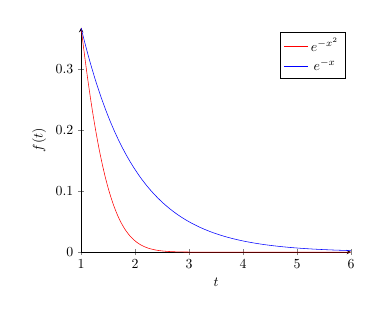
\begin{tikzpicture}[scale=0.5]
\centering
\begin{axis}[axis lines=left, xlabel=\(t\), ylabel=\(f(t)\)]
\addplot[domain=1:6, samples=200, color=red]{exp(-x^2)};
\addlegendentry{\(e^{-x^{2}}\)}
\addplot[domain=1:6, samples=200, color=blue]{exp(-x)};
\addlegendentry{\(e^{-x}\)}
\end{axis}
\end{tikzpicture}
\end{minipage}
\hfill
\begin{minipage}{0.7\linewidth}
For instance, the exponential random variable \(X \sim \mathrm{Exp}(\lambda)\) satisfies:
\begin{equation*}
\Pr(X > t) = e^{-\lambda t}
\end{equation*}

This doesn't decay as fast as the \emph{sub-Gaussian rate}, as shown in the plot on the right, and therefore is said to have a \emph{heavier} tail than a Gaussian.
\end{minipage}

Distributions such as these occur more commonly that just the exponential distribution in practice. For instance, let's consider the square of a sub-Gaussian random variable. Let \(Y = X^{2}\) where \(X\) is sub-Gaussian with sub-Gaussian norm \(\|X\|_{\psi_{2}} \leq K\). Then:
\begin{equation*}
\Pr(Y > t) = \Pr(|X| > \sqrt{t}) \leq 2\exp\left(-\frac{ct}{K^{2}}\right)
\end{equation*}
which shows that \(Y\) has a tail heavier than a sub-Gaussian. Such distributions are called \emph{Sub-Exponential distributions}. Below is a lemma similar to Lemma \ref{lem:sub-gauss-equiv} for sub-Exponential distributions that establishes equivalence properties.

\begin{lemma}
Let \(X\) be a sub-Exponential random variable. The following statements are equivalent:
\begin{description}
\item [(i)] \(\Pr(|X| > t) \leq 2\exp\left(-\frac{t}{K_{1}}\right)\) for all \(t \geq 0\)
\item [(ii)] \(\|X\|_{L^{p}} \leq K_{2}p\) for all \(p \geq 1\)
\item [(iii)] \(\Exp[\exp(\lambda|X|)] \leq \exp(K_{3}\lambda)\) for all \(\lambda \in \left[0, \frac{1}{K_{3}}\right]\)
\item [(iv)] \(\Exp\left[\exp\left(\frac{|X|}{K_{4}}\right)\right] \leq 2\)
\item [(v)] \(\Exp[\exp(\lambda X)] \leq \exp(K_{5}^{2}\lambda^{2})\) for all \(\lambda\) such that \(|\lambda| \leq \frac{1}{K_{5}}\)
\end{description}
\end{lemma}

\newpage
\bibliography{main}
\bibliographystyle{plainnat}
\end{document}
